\documentclass[10pt]{amsart}

\usepackage[T1]{fontenc}
\usepackage{amsmath,amssymb,amsthm}
\usepackage{graphicx}
\usepackage{float}
\usepackage{booktabs}
\usepackage[dvipsnames]{xcolor}
\usepackage[colorlinks=true,linkcolor=blue,citecolor=blue,urlcolor=blue]{hyperref}

\usepackage[left=2.1cm,right=2.1cm,top=2.9cm,bottom=2.9cm]{geometry}

\theoremstyle{definition}
\newtheorem{definition}{Definition}
\theoremstyle{remark}
\newtheorem{remark}{Remark}
\theoremstyle{plain}
\newtheorem{theorem}{Theorem}
\newtheorem{proposition}[theorem]{Proposition}
\newtheorem{corollary}[theorem]{Corollary}
\newtheorem{lemma}[theorem]{Lemma}

\newcommand{\R}{\mathbb{R}}
\newcommand{\N}{\mathbb{N}}
\DeclareMathOperator{\dist}{dist}

\begin{document}

\title{A PINNs approach for the computation of eigenvalues in elliptic problems}

\author{Juli\'an Fern\'andez Bonder}
\address{Departamento de Matem\'atica, Facultad de Ciencias Exactas y Naturales, Universidad de Buenos Aires, Buenos Aires, Argentina, and Instituto de C\'alculo UBA-CONICET, Buenos Aires, Argentina}
\email{jfbonder@dm.uba.ar}

\author{Ariel Salort}
\address{Departamento de Matem\'aticas Aplicadas y Ciencia de Datos, Universidad San Pablo-CEU, CEU Universities, Juli\'an Romea 2, 28003 Madrid, Spain}
\email{ariel.salort@ceu.es}


\begin{abstract}
We propose a physics-informed neural network (PINN) method for eigenvalue problems of elliptic
operators that relies neither on the Rayleigh quotient nor on orthogonality. For each value $E$ of the
spectral parameter, the squared residual of the equation is minimized over network functions that
satisfy the Dirichlet condition exactly, and the eigenvalues are detected as the minima of the
resulting loss curve. For self-adjoint operators the loss curve is the squared distance from $E$ to
the spectrum. For the penalized loss used in practice the loss curve is computed in closed form: it
has no spurious local minima and yields an explicit rule for the penalty parameter. The detection is
stable under training and sampling errors that are small compared with the squared spectral gaps,
and in the linear case every computed eigenvalue carries an a posteriori Weinstein and Kato--Temple
enclosure. For the $p$-Laplacian the zeros of the loss curve are exactly the eigenvalues and the
curve lies below a parabola at each of them. Experiments agree with exact values in dimensions two to four and with independent finite element
(dimensions two and three) and shooting computations, including $p$-Laplacian
eigenvalues beyond the second; in dimension ten, where mesh-based methods are not practical, the
method locates the first two eigenvalues to within $1\%$ (single run, weak certificate). The method
does not resolve multiplicities and, for the lowest eigenvalues of linear problems, it is more
expensive than Rayleigh-quotient methods with deflation.

\medskip\noindent\textbf{Keywords:} Physics-informed neural networks; eigenvalue problems; elliptic
PDEs; $p$-Laplacian; deep learning.

\noindent\textbf{AMS 2020 Classification:} 35P05, 35P30, 35J92, 65N25, 68T07.
\end{abstract}

\maketitle

% ===========================================================================
\section{Introduction}

Machine learning techniques are increasingly used to analyse problems governed by partial
differential equations (PDEs), and a growing number of software libraries support this use in
computational science and engineering; see, for instance,
\cite{Lu-Meng-Mao, Rackauckas, Rackauckas-Innes-Ma-Bettencourt-etal} and references therein.
Neural network-based solvers have been applied successfully to the Burgers, Eikonal and heat
equations \cite{Blechschmidt-Ernst}, to linear diffusion equations in complex two-dimensional
geometries \cite{Berg-Nystrom}, and to nonlinear problems such as three-dimensional PDEs,
Emden--Fowler systems and fractional-order predator--prey models \cite{GT24, KKG, MHO}. Nonlinear
dispersive models, such as the generalized higher-order nonlinear Schr\"odinger equation, whose
multi-peak and breather-type solitary waves were recently studied in \cite{Yasin-etal}, are further
natural targets for such solvers.

A prototypical problem is the eigenvalue problem of quantum mechanics,
\begin{equation}\label{eigen}
-\Delta u + V(x) u = E u,
\end{equation}
with a given potential $V$ and eigenvalue parameter $E\in\R$. In this paper it is posed in a bounded
domain $\Omega\subset\R^d$ with homogeneous Dirichlet boundary conditions. The use of neural networks
for such equations goes back to \cite{Lagaris-Likas-Fotiadis}, and gained momentum with
\emph{Physics-Informed Neural Networks} (PINNs) \cite{Raissi-Perdiakaris-Karniadakis}
(see also \cite{Karniadakis-etal}). Eigenvalue problems have been addressed in one dimension
\cite{Jin-Mattheakis-Protopapas1, Jin-Mattheakis-Protopapas2, Sakar}, in two dimensions
\cite{Holliday-Lindner-Ditto}, and for engineering and nonlinear problems
\cite{Rowan-Evans-Maute-Dootsan}; the Deep Ritz method \cite{E-Yu} also treats eigenvalue problems.
These approaches approximate $u$ by a fully connected network and minimize the \emph{Rayleigh quotient}
\[
R(u) = \frac{\int_{\Omega} |\nabla u|^2 + V(x) u^2\, dx}{\int_{\Omega} u^2\, dx},
\]
which yields the principal eigenpair; higher eigenpairs are obtained by minimizing again under
orthogonality (deflation) constraints against the previously computed eigenfunctions. This has two
limitations: it is sequential (to reach an eigenvalue one must compute all the lower ones, and
their errors propagate), and it does not extend to nonlinear operators such as the $p$-Laplacian,
where no orthogonality between eigenfunctions is available.

\emph{The idea.} We fix $E$ and minimize the squared residual $\|(-\Delta+V-E)u\|^2/\|u\|^2$ over
network functions. The minimal value, as a function of $E$, is a \emph{loss curve} that vanishes
exactly at the eigenvalues. Scanning $E$ and locating the minima of this curve detects the
eigenvalues in a prescribed window without the Rayleigh quotient and without orthogonality, and the
same mechanism applies verbatim to nonlinear eigenvalue problems.

\emph{Contributions.} (i) For self-adjoint problems the loss curve is $\Lambda(E)=\dist(E,\sigma)^2$
(Section~\ref{sec.approach}). (ii) The loss curve of the penalized loss used in practice is computed in
closed form; it has no spurious local minima and gives the rule $\mu\ge D^2$ for the penalty parameter
(Proposition~\ref{prop.penalized}, Corollary~\ref{cor.mu}). (iii) Every computed eigenvalue carries an
a posteriori Weinstein and Kato--Temple enclosure (Section~\ref{sec.certificate}), and the detection is
stable under training and sampling errors that are small compared with the squared gaps
(Proposition~\ref{prop.stability}); we measure this error level. (iv) We validate the method against
exact values in dimensions $2$--$4$ and independent finite element computations in
dimensions $2$ and $3$, test it in
dimension $10$ (Section~\ref{sec.examples}), and compare its cost with a Rayleigh-quotient PINN with
deflation (Section~\ref{sec.cost}). (v) For the $p$-Laplacian, the zeros of the loss curve are exactly
the eigenvalues and $\Lambda_p(E)\le\inf_kc_k(E-E_k)^2$; we compute eigenvalues beyond the second
one and compare them with independent references (Section~\ref{sec.nolin}).

\emph{Organization.} Section~\ref{sec.approach} presents the method and its analysis,
Section~\ref{sec.examples} the linear experiments, Section~\ref{sec.nolin} the $p$-Laplacian,
Section~\ref{sec.cost} the cost, and Section~\ref{sec.conclusions} the conclusions and limitations.
Proofs are collected in Appendix~\ref{app.proofs}, implementation details in
Appendix~\ref{sec.implementation}, and further experiments and studies in
Appendices~\ref{app.linear}--\ref{app.plap}.

% ===========================================================================
\section{The method}\label{sec.approach}

\subsection{The loss curve}
For $u\ne0$ and $E\in\R$ let
\begin{equation}\label{Lambda}
\Lambda(u, E) = \frac{\int_{\Omega} (\Delta u - V(x) u + Eu)^2\, dx}{\int_{\Omega} u^2\, dx},
\qquad
\Lambda(E) = \inf_u \Lambda(u, E).
\end{equation}
We call $E\mapsto\Lambda(E)$ the \emph{loss curve}. A minimizer exists (Theorem~\ref{teo.min}).

Let $L=-\Delta+V$, with the Dirichlet condition built into its domain $\mathrm{Dom}(L)$, be
self-adjoint with compact resolvent (this is the case for a bounded domain and bounded $V$), let
$E_1\le E_2\le\cdots$ be its eigenvalues repeated according to multiplicity, $\{u_k\}$ an orthonormal
basis of eigenfunctions, $\sigma=\{E_k\}$ the spectrum and $\ell(E):=\dist(E,\sigma)$. Writing $u=\sum_ka_ku_k\in \mathrm{Dom}(L)$,
\[
\Lambda(u,E)=\frac{\sum_k a_k^2 (E_k-E)^2}{\sum_k a_k^2}\ \ge\ \min_k (E_k-E)^2,
\]
with equality if and only if $u$ lies in the eigenspace of the eigenvalue(s) closest to $E$. Hence
\begin{equation} \label{cota.igual}
\Lambda(E)=\min_k (E_k-E)^2=\ell(E)^2 .
\end{equation}
Thus $\Lambda\ge0$, the zeros of $\Lambda$ are exactly the eigenvalues, every local minimum of
$\Lambda$ is a zero, and $\Lambda$ is a parabola of unit curvature around each eigenvalue
(Fig.~\ref{Lambda.fig}). The curve does not see multiplicities: a multiple eigenvalue produces a
single zero.

The characterization of the eigenvalues as the zeros of $\Lambda$ uses only that $\Lambda(u,E)$ is
the squared residual of the equation, not the spectral decomposition. For nonlinear problems the
identity \eqref{cota.igual} is lost, but the loss still vanishes exactly at the eigenvalues and lies
below a parabola near each of them (Proposition~\ref{prop.plap}). Scanning a spectral parameter and
locating the minima of a residual is classical in other contexts (the method of particular solutions
\cite{Betcke-Trefethen}, the folded-spectrum method \cite{Wang-Zunger}); here it is combined with a
neural network ansatz, which makes it applicable in several dimensions and to nonlinear operators.
The loss at a given $E$ does not involve any other eigenpair: no orthogonalization is needed and
errors in one eigenvalue do not propagate to the next.

\begin{figure}[tbp]
\centering
\begin{minipage}[t]{.47\textwidth}
\centering
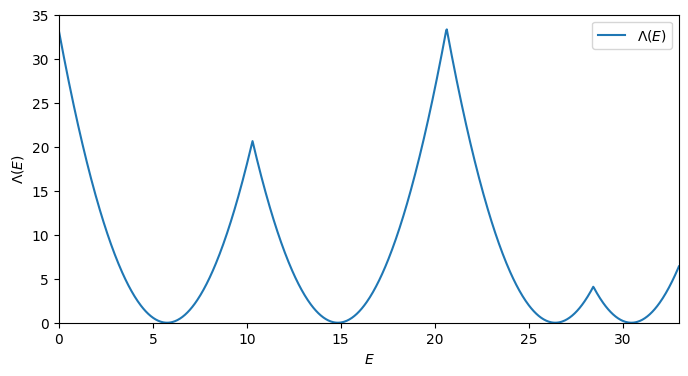
\includegraphics[width=.9\textwidth]{Loss.png}
\caption{The exact loss curve $\Lambda(E)=\min_k(E-E_k)^2$ for the Dirichlet Laplacian in the unit
disk; the first four distinct eigenvalues are $E_1 = 5.7832$, $E_2 = 14.6820$, $E_3 = 26.3746$,
$E_4 = 30.4713$ ($E_2$ and $E_3$ are double).}
\label{Lambda.fig}
\end{minipage}\hfill
\begin{minipage}[t]{.47\textwidth}
\centering
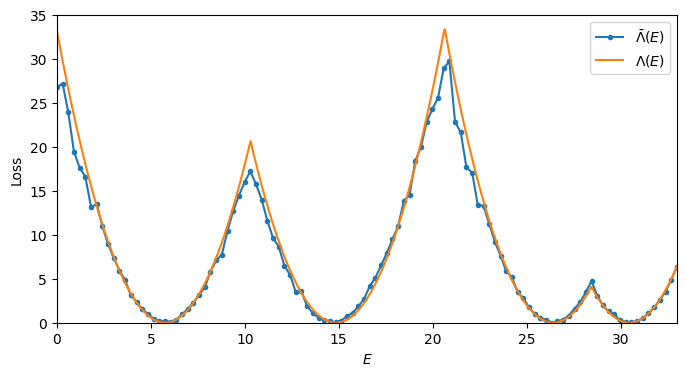
\includegraphics[width=.9\textwidth]{lossNN-lento.png}
\caption{The computed loss curve $\bar\Lambda(E)$ in the unit disk ($\mu=100$) compared with the
exact curve $\Lambda(E)$; near the peaks the penalized curve lies below $\Lambda(E)$, as predicted
by Proposition~\ref{prop.penalized}.}
\label{lossNN.fig}
\end{minipage}
\end{figure}

\subsection{The penalized loss and the choice of \texorpdfstring{$\mu$}{mu}}
The networks are of the form $u=B\,\mathrm{NN}_\theta$, where $B$ is a smooth factor vanishing exactly
on $\partial\Omega$, so that the Dirichlet condition holds exactly and every network function lies in
$\mathrm{Dom}(L)$ (Appendix~\ref{sec.implementation}). The normalization is enforced by a penalty:
\begin{equation}\label{lossmu}
\bar \Lambda(u, E) = \int_\Omega (\Delta u -Vu + Eu)^2\, dx + \mu\left(\int_\Omega u^2\, dx - 1\right)^2,
\end{equation}
with the integrals approximated by Monte Carlo sample means. The penalized loss curve is explicit.

\begin{proposition}[Loss curve of the penalized loss]\label{prop.penalized}
Let $\mu>0$, $E\in\R$ and $\ell=\ell(E)$. Then
\[
\bar\Lambda(E):=\inf_{u\in \mathrm{Dom}(L)}\bar\Lambda(u,E)=
\begin{cases}
\ell^2-\dfrac{\ell^4}{4\mu} & \text{if } \ell^2\le 2\mu,\\[2mm]
\mu & \text{if } \ell^2\ge 2\mu .
\end{cases}
\]
If $\ell^2<2\mu$ the minimizers are the functions $u$ in the eigenspace(s) of the eigenvalue(s)
closest to $E$ with $\|u\|_2^2=1-\ell^2/(2\mu)$; for them $\Lambda(u,E)=\ell^2$ and the residual term
equals $\ell^2(1-\ell^2/(2\mu))$. If $\ell^2\ge2\mu$ the unique minimizer is $u=0$. Moreover, for every $E$
all local minimizers of $\bar\Lambda(\cdot,E)$ in $\mathrm{Dom}(L)$ are global minimizers, and every other
critical point is a saddle point.
\end{proposition}

Thus the continuous landscape has no spurious local minima, the zeros of $\bar\Lambda$ are exactly
the eigenvalues for every $\mu>0$, and the only artifact of the penalty is the trivial state $u=0$
when $\ell(E)^2\ge2\mu$. Spurious minima observed in practice can only come from the network
parametrization, the optimizer or the sampling. Let $[E_*,E^*]$ be the window of the scan,
$D=\max_{E\in[E_*,E^*]}\ell(E)$ (half of the largest gap meeting the window, or the distance from an
endpoint to the spectrum if larger), and $\mathcal R_\mu(E)$ the residual term of \eqref{lossmu} at the
minimizer, which is the quantity recorded during the scan.

\begin{corollary}\label{cor.mu}
(i) For every $\mu>0$ the zeros of $\bar\Lambda(E)$ are exactly the eigenvalues, and
$0\le \ell^2-\bar\Lambda(E)\le \ell^4/(4\mu)$ when $\ell^2\le2\mu$. (ii) If $\mu\ge D^2$, then
$\|u_E\|_2^2\ge\frac12$ and $\mathcal R_\mu(E)=\ell^2(1-\ell^2/(2\mu))$ is an increasing function of $\ell=\ell(E)$ on the
window: its zeros and local minima are exactly the eigenvalues. (iii) If $\frac12D^2\le\mu<D^2$,
$\mathcal R_\mu$ has spurious local minima where $\ell$ has a local maximum larger than $\sqrt\mu$. (iv) If
$\mu<\frac12D^2$, the minimizer is $u_E=0$ wherever $\ell(E)^2\ge2\mu$, and the recorded curve has
spurious zeros there.
\end{corollary}

\emph{Guideline.} Along a warm-started scan take $\mu\ge D^2$ (we recommend $\mu\approx2D^2$);
$D$ can be estimated from Weyl's law or from a coarse preliminary scan, and since the gaps do not
grow with $E$ in dimension $d\ge2$, $\mu$ need not grow with $E$. A very large $\mu$ is harmful (noise
floor $\mu\operatorname{Var}(u^2)/N$, stiffness). In a test on a window of the unit square containing
two eigenvalues, the recorded residual had a spurious minimum in the gap in all six runs with
$\mu<D^2$ and in none of the six runs with $\mu\ge D^2$, and the networks collapsed to $u=0$ exactly at
the predicted nodes for $\mu<D^2/2$ (Appendix~\ref{sec.mu}, Table~\ref{table.mu}). Training from
scratch at a high value of $E$ is a different matter: it is unreliable, and high windows are reached
by warm-start continuation from below (Appendix~\ref{sec.analysis}).

\begin{table}[tbp]
\centering\small
\caption{Test of the rule $\mu\ge D^2$: window $[15,55]$ of the unit square ($D^2=219.2$; the value $\mu=219$ is $\approx D^2$), offset grid of 16 nodes, two seeds, reduced network. Spurious minima: interior local minima of the recorded residual more than $2.5$ away from an eigenvalue, seed 0 / seed 1. Collapsed: nodes with $\overline{u^2}<0.1$, observed / predicted by Proposition~\ref{prop.penalized}. $\hat E$: Rayleigh quotient near $5\pi^2=49.3480$ (seeds 0, 1).}
\label{table.mu}
\begin{tabular}{rrcccc}
\toprule
$\mu$ & $\mu/D^2$ & regime & spurious minima & collapsed & $\hat E$\\
\midrule
30 & 0.14 & (iv) & 3 / 1 ($E=28$--$41$) & 6/6 & 49.3482, 49.3477\\
75 & 0.34 & (iv) & 1 / 1 ($E=33$--$36$) & 2/2 & 49.3487, 49.3476\\
150 & 0.68 & (iii) & 1 / 1 ($E=35.6$) & 0/0 & 49.3473, 49.3478\\
219 & $\approx1.0$ & (ii) & none & 0/0 & 49.3487, 49.3483\\
300 & 1.4 & (ii) & none & 0/0 & 49.3479, 49.3481\\
1000 & 4.6 & (ii) & none & 0/0 & 49.3475, 49.3475\\
\bottomrule
\end{tabular}
\end{table}

\subsection{The algorithm}
Fix a window $[E_*,E^*]$ and a grid $E_*=E^1<\cdots<E^J=E^*$. The grid need not be uniform (it can,
for instance, be refined near candidate minima); for simplicity we use a uniform step $h$, and the
stability result below is stated in that case. For each $E^i$ the
network is trained to minimize $\bar\Lambda(\cdot,E^i)$, initialized with the weights obtained at
$E^{i-1}$ (warm start). At each node we record the normalized loss $\Lambda(u^i,E^i)$, the mass
$\overline{u^2}$ and the Rayleigh quotient, and discard nodes with $\overline{u^2}<\frac12$ (collapse to
$u=0$). The local minima of the discrete curve are the detected eigenvalues; each is refined from the
trained network as described next, and the network approximates the eigenfunction.

\subsection{Refinement and a posteriori enclosure}\label{sec.certificate}
For $u\in \mathrm{Dom}(L)\setminus\{0\}$ (for instance a trained network) let
\[
r(u,E)=\frac{\|(L-E)u\|_2}{\|u\|_2}=\Lambda(u,E)^{1/2},\qquad
\rho(u)=\frac{\langle Lu,u\rangle}{\|u\|_2^2},\qquad \eta(u)=r(u,\rho(u)).
\]

\begin{proposition}\label{prop.rayleigh}
Let $u\in \mathrm{Dom}(L)\setminus\{0\}$. Then:
\begin{enumerate}
\item[(a)] $\Lambda(u,E)=(E-\rho(u))^2+\eta(u)^2$ for every $E\in\R$; in particular, for fixed $u$ the
minimum of $E\mapsto\Lambda(u,E)$ is attained at the Rayleigh quotient $\rho(u)$.
\item[(b)] (Weinstein \cite{Weinstein1934,Parlett1998}) $\ell(E)\le r(u,E)$ for every $E$: the interval
$[E-r,E+r]$ contains an eigenvalue of $L$.
\item[(c)] (Kato--Temple \cite{Kato1949,Parlett1998}) If $E_k$ is the only eigenvalue of $L$ in
$(\rho(u)-\gamma,\rho(u)+\gamma)$, then $|\rho(u)-E_k|\le\eta(u)^2/\gamma$.
\end{enumerate}
\end{proposition}

\emph{Refinement.} Once a minimum $E^{i_0}$ is detected, the network $u^{i_0}$ is frozen and the
eigenvalue is taken as the minimizer of $E\mapsto\Lambda(u^{i_0},E)$, which by (a) is
\[
\hat E=\rho(u^{i_0})=-\frac{\int_\Omega u^{i_0}(\Delta u^{i_0}-Vu^{i_0})\,dx}{\int_\Omega (u^{i_0})^2\,dx}.
\]
No further training is needed, and the accuracy does not depend on the grid step $h$; all the
eigenvalues reported in this paper are computed in this way (estimators compared in
Appendix~\ref{app.refine}).

\emph{Certificate.} Items (b) and (c) hold for \emph{any} $u\in \mathrm{Dom}(L)$, whatever the quality of
the training. Hence each detection comes with the enclosure $|E-E_k|\le r$ and, if $\gamma$ is a lower
bound for the distance to the rest of the spectrum (obtainable from the enclosures of the
neighbouring detections), with $|\hat E-E_k|\le\eta^2/\gamma$. The eigenvalue error is therefore
\emph{quadratic} in the residual: $\eta^2=10^{-1}$ and $\gamma=10$ guarantee an error at most
$10^{-2}$, although $\eta\approx0.32$. This explains the pattern observed in all our tables: accurate
eigenvalues together with comparatively large residuals. In the tables, $\mathrm{Residual}$ is the
sampled first term of \eqref{lossmu} and $r=(\mathrm{Residual}/\overline{u^2})^{1/2}$ the Weinstein
radius. Since the integrals are evaluated by Monte Carlo, the certificate is statistical; with
$4\times10^5$ points the standard error of $r$ was $0.1$--$0.4\%$ of $r$
(Appendix~\ref{app.refine}).

\emph{Upper bound for $E_1$.} A network function vanishes on $\partial\Omega$ and is smooth, so
integration by parts gives $\rho(u)=R(u)\ge E_1$ (Rayleigh--Ritz): the computed first eigenvalue is
an upper bound for $E_1$, up to the Monte Carlo error. If a lower bound $\beta\le E_2$ with
$\rho(u)<\beta$ is available, Temple's inequality \cite{Kato1949} gives the bracket
$\rho(u)-\eta(u)^2/(\beta-\rho(u))\le E_1\le\rho(u)$. For higher eigenvalues the error is quadratic in the
components of $u$ outside the eigenspace and positive when these lie mainly in higher modes; most of
the differences we observed are positive (Appendix~\ref{app.refine}).

\subsection{Stability of the detection}\label{sec.stability}
The identity \eqref{cota.igual} concerns exact minimizers, whereas the network class
$\mathcal N=\{B\,\mathrm{NN}_\theta\}$ is finite dimensional, training stops after finitely many steps,
and the integrals are sampled. Since $\mathcal N\subset\mathrm{Dom}(L)$, approximation and optimization
errors can only raise the loss curve. Let $\tilde\Lambda_i$ be the computed normalized loss at the node
$E^i=E_*+(i-1)h$; we assume only a bound on the total error,
\begin{equation}\label{hyp.delta}
|\tilde\Lambda_i-\ell(E^i)^2|\le\delta,\qquad i=1,\dots,J,
\end{equation}
and call an interior node $E^m$ a discrete local minimum if
$\tilde\Lambda_m\le\min\{\tilde\Lambda_{m-1},\tilde\Lambda_{m+1}\}$.

\begin{proposition}[Stability of the loss-curve characterization]\label{prop.stability}
Assume \eqref{hyp.delta}, let $\epsilon>0$ be the detection threshold and
$\tau=\sqrt{h^2/4+2\delta}$.
\begin{enumerate}
\item[(a)] (No detections away from the spectrum.) If $\tilde\Lambda_i\le\epsilon$, then
$\ell(E^i)\le\sqrt{\epsilon+\delta}$.
\item[(b)] (No missed eigenvalues by thresholding.) Every eigenvalue $E_k\in[E_*,E^*]$ has a node
with $|E^i-E_k|\le h/2$ and $\tilde\Lambda_i\le h^2/4+\delta$; hence all of them are detected if
$\epsilon\ge h^2/4+\delta$.
\item[(c)] (Local minima are close to the spectrum.) Every discrete local minimum satisfies
$\ell(E^m)\le\max\{h,\ h/2+\delta/h\}$, irrespective of its value.
\item[(d)] (Isolated eigenvalues produce local minima.) If
$[E_k-\tau-h,E_k+\tau+h]\subset[E_*,E^*]$ and $\dist(E_k,\sigma\setminus\{E_k\})>2\tau+h$, there is a
discrete local minimum $E^m$ with $|E^m-E_k|\le\tau$.
\end{enumerate}
\end{proposition}

Imperfect training therefore cannot create detections far from the spectrum; it can only produce
several minima near one eigenvalue, or raise the curve so that an eigenvalue is missed. Part (d)
applies when $\delta\ll\gamma^2/8$, $\gamma$ the gap. We do not prove a bound on $\delta$, but it can
be \emph{measured}: in the unit square, on all nodes that had neither collapsed nor switched branch,
$\delta\le12.1$, well below $\gamma^2/8=48.7$ and $109.6$ for the gaps $19.7$ and $29.6$, and the
hypotheses of (d) hold. Collapsed and branch-switched nodes are visible in the network itself (vanishing
mass, jump of the Rayleigh quotient); see Appendix~\ref{sec.analysis} and Remark~\ref{rem.stability}.

% ===========================================================================
\section{Linear examples}\label{sec.examples}

We use a $3\times128$ $\tanh$ network times the boundary factor $B$, Adam with learning rate
$10^{-3}$, $N=5000$ fresh Monte Carlo points per epoch, and warm start along the grid; the settings of
every example (window, step, $\mu$, epochs, seeds, regime of $\mu$) are listed in
Table~\ref{table.settings} (Appendix~\ref{sec.implementation}). The code, the scripts and the raw
results are available in the repository given in the Declaration. We begin with the hard-wall
potential ($V=0$ in $\Omega$), i.e.\ the Dirichlet Laplacian
\begin{equation}\label{eigen2}
-\Delta u = E u \ \text{ in }\Omega,\qquad u=0\ \text{ on }\partial\Omega.
\end{equation}

\subsection{Exact eigenvalues: disk and square}
Fig.~\ref{lossNN.fig} shows the computed curve in the unit disk; the eigenfunctions are in
Fig.~\ref{func.fig}. Table~\ref{table.1} reports a scan of $[0,105]$ in the unit square (80 nodes,
$\mu=500$, re-initialization every 25 nodes). All rows satisfy the Weinstein bound $|\hat E-E_k|\le r$,
with errors two to four orders of magnitude below $r$, as predicted by the quadratic error of the
Rayleigh quotient. The double eigenvalues appear as single minima.

\begin{table}[tbp]
\centering\small
\caption{Eigenvalues of problem \eqref{eigen2} in the unit square $[0,1]\times[0,1]$ compared with the exact values (scan of $[0,105]$ with 80 nodes, $\mu=500$, seed 0; $E$ is the Rayleigh quotient of the trained network evaluated on a $300\times300$ midpoint grid; Residual is evaluated on a fresh Monte Carlo sample at the reported $E$; $r=(\mathrm{Residual}/\overline{u^2})^{1/2}$ is the Weinstein radius). The double eigenvalues $5\pi^2$ and $10\pi^2$ appear as a single minimum; the multiplicity is not detected by the method.}
\label{table.1}
\begin{tabular}{ccccccc}
\toprule
$(m,n)$ & mult. & $E_{(m,n)}=\pi^2(m^2+n^2)$ & Our method & Rel.\ error & Residual & $r$ \\
\midrule
$(1,1)$ & 1 & $2\pi^2\approx 19.7392$ & 19.739909 & $3.5\times10^{-5}$ & $9.7\times10^{-2}$ & 0.31\\
$(1,2),(2,1)$ & 2 & $5\pi^2\approx 49.3480$ & 49.348167 & $2.9\times10^{-6}$ & $7.3\times10^{-2}$ & 0.27\\
$(2,2)$ & 1 & $8\pi^2\approx 78.9568$ & 78.956161 & $8.5\times10^{-6}$ & $2.0\times10^{-1}$ & 0.44\\
$(1,3),(3,1)$ & 2 & $10\pi^2\approx 98.6960$ & 98.695973 & $7.2\times10^{-7}$ & $9.3\times10^{-2}$ & 0.30\\
\bottomrule
\end{tabular}
\end{table}

\begin{figure}[tbp]
\centering
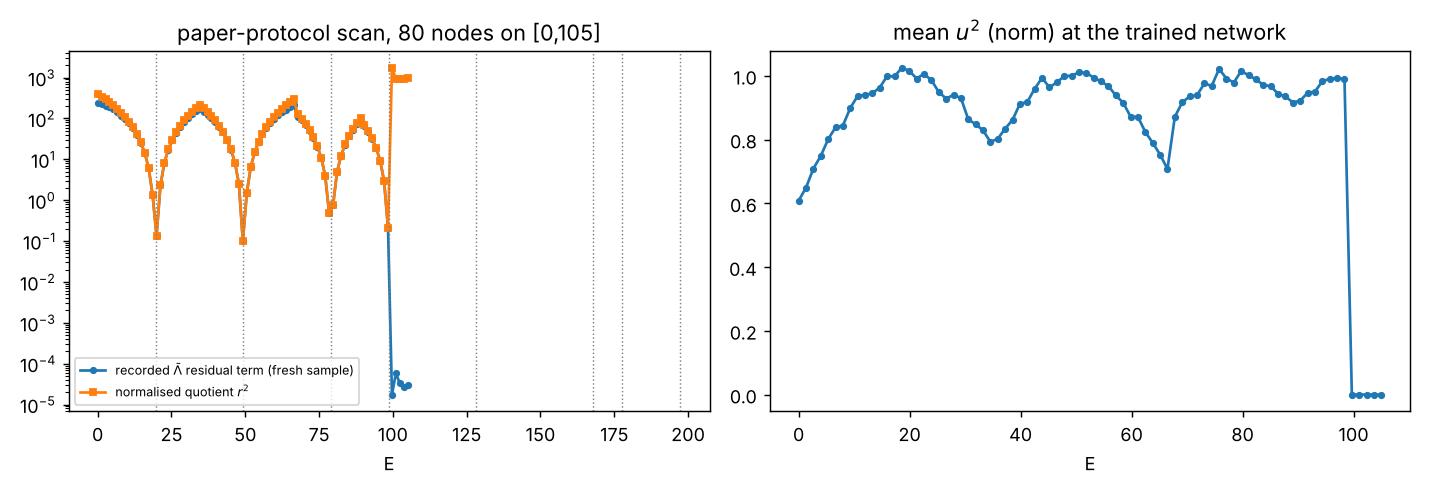
\includegraphics[width=.6\textwidth]{paper_sweep_curve.png}
\caption{The scan of Table~\ref{table.1} (80 nodes on $[0,105]$, $\mu=500$). Left: recorded residual term and normalized loss $r^2$ (dotted lines: eigenvalues). Right: mean of $u^2$. After the re-initialization at $E=99.7$ the network collapses to $u\equiv0$: the recorded residual drops to $10^{-5}$ while $r^2$ jumps to $\approx10^3$.}
\label{fig.collapse}
\end{figure}

The results are reproducible and the certificates are informative. On the window $[15,55]$ of the
square (step 5, $\mu=450$), seeds 0, 1, 2 all gave local minima at $E=20$ and $E=50$ only, with refined
values $19.7394$, $19.7397$, $19.7450$ for $2\pi^2$ and $49.3486$, $49.3485$, $49.3474$ for $5\pi^2$. Over
the 14 minima detected in our unit-square runs the Weinstein radius exceeded the actual error by a
factor $120$--$4300$ and the Kato--Temple bound by a factor $2.7$--$66$ (median $7.5$): both bounds held,
and the Kato--Temple bound is the informative one. The only spurious zeros of the recorded curve were
collapses to $u\equiv0$ after a re-initialization at $E=99.7$, immediately flagged by
$\overline{u^2}\approx10^{-8}$ and $r=30$--$42$ (Fig.~\ref{fig.collapse}, Appendix~\ref{sec.analysis}).

\subsection{A potential: comparison with finite elements}\label{sec.fem}
For potentials no closed-form eigenvalues are available, and we compare with independent finite
element (FEM) reference values ($P_2$ isoparametric elements, Richardson extrapolation; details in
Appendix~\ref{app.fem}). We take the double-well Gaussian potential in the unit ball of $\R^3$,
\[
V(x)=-e^{-2|x-e_1|^2}-e^{-2|x+e_1|^2},\qquad e_1=(1,0,0),
\]
whose wells are centred on the boundary sphere. Table~\ref{table.blind} reports a \emph{blind} scan of
$[4.7,49.7]$ with a grid not aligned with the spectrum. The interval contains $11$ distinct FEM
eigenvalues ($17$ with multiplicity) in five clusters; the loss curve has exactly five local minima,
one per cluster, every FEM eigenvalue lies within $0.75$ of one of them, and the Rayleigh quotient is
within $0.04\%$ of the nearest FEM eigenvalue. On windows centred at the FEM values, with 2--3 seeds,
the seed means agree with FEM to within $0.1\%$ and single runs to within $0.25\%$ for the double-well,
four-well and harmonic potentials (Table~\ref{table.fem}; the four-well and harmonic potentials are
defined in Appendix~\ref{sec.potentials}), although $\min\Lambda$
is $0.06$--$1.05$ (i.e.\ $r=0.25$--$1$): the accuracy comes from the Rayleigh quotient. The loss curve
has one minimum per cluster of close eigenvalues and the quotient returns a value inside the cluster;
the number and multiplicities of the eigenvalues in a cluster cannot be read from the curve. For these
linear problems in low dimension FEM is much cheaper and more accurate: a 7-point PINN window took
$7$--$25$ minutes on one CPU core, the FEM computation of all eigenvalues in $[0,75]$ less than $10$\,s in
two dimensions and about $2$ minutes for the ball of $\R^3$.

\begin{table}[tbp]
\centering\small
\caption{Blind scan of the double well (unit ball of $\R^3$, $E=4.7,6.2,\dots,49.7$, $\mu=400$, seed 0): local minima of the recorded loss, Rayleigh quotient $\hat E$ of the network at the minimum, finite element eigenvalues within $1.5$ (multiplicity), and relative difference of $\hat E$ to the nearest one.}
\label{table.blind}
\begin{tabular}{cccc}
\toprule
minimum at $E$ & $\hat E$ & FEM eigenvalues within $1.5$ & rel.\ diff.\ (\%)\\
\midrule
9.2 & 9.5779 & 9.576 (1) & $+0.015$\\
19.7 & 19.7545 & 19.752 (1), 19.967 (2) & $+0.012$\\
33.2 & 32.7966 & 32.786 (1), 32.874 (2), 33.034 (2) & $+0.034$\\
39.2 & 39.1945 & 39.192 (1) & $+0.005$\\
48.2 & 48.5270 & 48.406 (1), 48.430 (2), 48.545 (2), 48.676 (2) & $-0.038$\\
\bottomrule
\end{tabular}
\end{table}

\begin{table}[tbp]
\centering\footnotesize
\caption{PINN versus finite elements (FEM) for the potentials of Appendix~\ref{sec.potentials}. FEM: extrapolated value $\pm$ estimated uncertainty (multiplicity); $^\dagger$: other FEM eigenvalues within $0.75$, i.e.\ a cluster that the scan does not resolve (the reference is then the cluster member nearest to the computed value). $\hat E$: Rayleigh quotient of the trained network for each seed. Rel.\ diff.: of the seed mean, and largest over single seeds.}
\label{table.fem}
\begin{tabular}{@{}lllccc@{}}
\toprule
example & FEM (mult.) & $\hat E$ per seed & \multicolumn{2}{c}{rel.\ diff.\ (\%)} & $\min\Lambda$\\
 & & & mean & worst & \\
\midrule
double well, ball $\R^3$ & $9.5764\pm0.0005$ (1) & 9.5783, 9.5782 & $+0.019$ & 0.019 & 0.065\\
 & $19.7522\pm0.003$ (1)$^\dagger$ & 19.7640, 19.7547 & $+0.036$ & 0.060 & 0.077\\
 & $32.8735\pm0.02$ (2)$^\dagger$ & 32.9552, 32.8571 & $+0.099$ & 0.248 & 0.117\\
 & $39.1924\pm0.01$ (1) & 39.1944, 39.1938 & $+0.004$ & 0.005 & 0.108\\
\midrule
four well, ball $\R^3$ & $9.8542\pm0.0005$ (1) & 9.8593, 9.8646, 9.8581 & $+0.066$ & 0.105 & 0.355\\
 & $20.1801\pm0.003$ (2)$^\dagger$ & 20.1505, 20.1878, 20.1870 & $-0.025$ & 0.147 & 0.478\\
 & $33.2104\pm0.01$ (2)$^\dagger$ & 33.2141, 33.2077, 33.2061 & $-0.003$ & 0.013 & 0.407\\
 & $39.4573\pm0.01$ (1) & 39.4578, 39.4414, 39.4554 & $-0.015$ & 0.040 & 1.054\\
\midrule
harmonic $\omega=10$, disk & $14.2847$ (1) & 14.2899, 14.2904 & $+0.038$ & 0.040 & 0.174\\
 & $29.1349$ (2) & 29.1357, 29.1353 & $+0.002$ & 0.003 & 0.056\\
 & $45.0887$ (2) & 45.0892, 45.0892 & $+0.001$ & 0.001 & 0.065\\
 & $62.5793$ (2) & 62.5792, 62.5800 & $+0.0005$ & 0.001 & 0.076\\
\bottomrule
\multicolumn{6}{@{}l}{FEM uncertainties for $\omega=10$ (two dimensions): $3\times10^{-7}$--$2\times10^{-5}$.}
\end{tabular}
\end{table}

\subsection{Balls of \texorpdfstring{$\R^3$}{R3} and \texorpdfstring{$\R^4$}{R4}}
In the unit ball $B^d$, $d=3,4$, the eigenvalues are known explicitly: for $m\in\N_0$, $n\in\N$,
$E_{(m,n)}=j_{m+\frac12,n}^2$ with multiplicity $2m+1$ if $d=3$, and $E_{(m,n)}=j_{m+1,n}^2$ with
multiplicity $(m+1)^2$ if $d=4$, where $j_{\nu,n}$ is the $n$-th positive zero of the Bessel function
$J_\nu$. Fig.~\ref{loss3D.fig} shows full scans starting at $E=0$ ($\mu=100$ for $d=3$ and $\mu=200$ for
$d=4$). To measure the accuracy we trained, for each of the first eigenvalues, on three nodes $E_k-0.9$,
$E_k+0.1$, $E_k+1.1$ (fresh network at the first node, warm start at the other two, seed 0, settings of
Table~\ref{table.settings}) and report the Rayleigh quotient at the node of smallest normalized loss
(Table~\ref{table.2}). These windows were placed using the known eigenvalues: they test the accuracy of
the computed values, not their detection. In $\R^3$ already the first (cold) node converged to the
targeted eigenfunction ($|\hat E-E_k|\le0.01$, $r\approx1$). In $\R^4$ the quotient still follows the
training value across the window ($14.507$, $14.712$, $14.963$ at $E=13.78$, $14.78$, $15.78$): with 2000
epochs the network has not fully converged to an eigenfunction, and the quotient is reliable only at
the node of smallest loss.

\begin{table}[tbp]
\centering\small
\caption{Eigenvalues of \eqref{eigen2} in the unit balls of $\R^3$ and $\R^4$ (three-node windows, seed 0). $\hat E$: Rayleigh quotient at the node of smallest normalized loss, with its Monte Carlo standard error in the last digits ($4\times10^5$ points); $r$: Weinstein radius. In $\R^4$ the quotient drifts with the node ($14.51$, $14.71$, $14.96$ for the first eigenvalue); the value at the node of smallest loss is given. The higher eigenvalues in the windows of Fig.~\ref{loss3D.fig} were not recomputed in this way and are shown only in that figure.}
\label{table.2}
\begin{tabular}{ccccccc}
\toprule
$d$ & $(m,n)$ & mult. & $E_{(m,n)}$ & $\hat E$ & rel.\ error & $r$\\
\midrule
3 & $(0,1)$ & 1 & $j_{1/2,1}^2\approx9.8696$ & 9.8757(4) & $6.2\times10^{-4}$ & 0.41\\
3 & $(1,1)$ & 3 & $j_{3/2,1}^2\approx20.1907$ & 20.1912(4) & $2.2\times10^{-5}$ & 0.22\\
3 & $(2,1)$ & 5 & $j_{5/2,1}^2\approx33.2175$ & 33.2178(4) & $9\times10^{-6}$ & 0.26\\
3 & $(0,2)$ & 1 & $j_{1/2,2}^2\approx39.4784$ & 39.4789(6) & $1.3\times10^{-5}$ & 0.24\\
\midrule
4 & $(0,1)$ & 1 & $j_{1,1}^2\approx14.6820$ & 14.7122(5) & $2.1\times10^{-3}$ & 0.46\\
4 & $(1,1)$ & 4 & $j_{2,1}^2\approx26.3746$ & 26.3980(10) & $8.9\times10^{-4}$ & 0.79\\
\bottomrule
\end{tabular}
\end{table}

\begin{figure}[tbp]
\centering
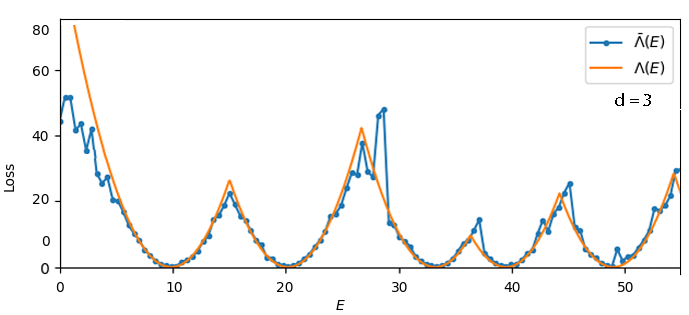
\includegraphics[width=.4\columnwidth]{loss_n=3_V=0_p=2_mu=100_reseteo_cada_15_iteraciones.png}
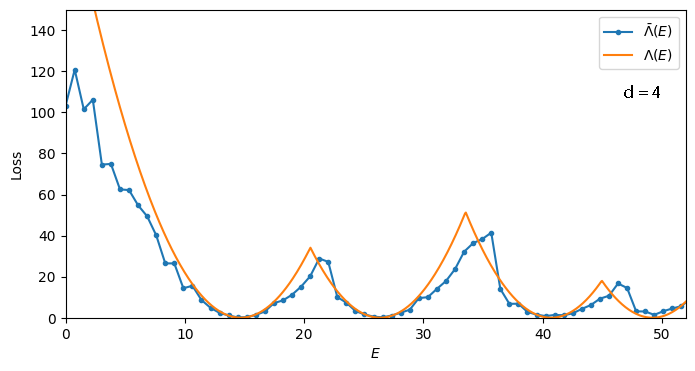
\includegraphics[width=.4\columnwidth]{loss_n=4_p=2_V=0_mu=200.png}
\caption{The loss curve $\bar\Lambda(E)$ in the unit ball of $\R^3$ (left) and of $\R^4$ (right) compared with the exact curve.}
\label{loss3D.fig}
\end{figure}


\subsection{Dimension ten}\label{sec.d10}
The cost of an epoch grows only linearly with $d$ (about $60+50d$ ms per epoch for the $3\times128$
network with 5000 points on one thread), whereas mesh-based methods become infeasible in high
dimension. We scanned the unit ball of $\R^{10}$, whose first eigenvalue $j_{4,1}^2=57.583$ is simple and
whose second, $j_{5,1}^2=76.939$, has multiplicity 10, on the nodes $E=54,57,\dots,84$, a window chosen
around the known eigenvalues (warm start, at most 2000 epochs, a single run with seed 0; 1.8 hours on
one thread). Most of the volume of this ball lies near its boundary, where $B=1-|x|^2$ is small; with
$\mu=200$ the network collapsed to $u\equiv0$ at the first node, and we used $\mu=2000$. The recorded
residual has two wells (19.8 at $E=57$ and 49.4 at $E=78$, against 234 at $E=72$), the tenfold eigenvalue
appearing as a single minimum. The Rayleigh quotient depends on the node: it is $57.62$--$57.84$ at the
nodes of the first well ($+0.07\%$ to $+0.45\%$) and $77.10$--$77.70$ at those of the second ($+0.2\%$ to
$+1.0\%$); no Monte Carlo standard error was computed for this run. With $r\approx4.7$--$7$ at the minima
the Weinstein enclosure is weak, so this example shows feasibility rather than accuracy.

\subsection{Other examples}
Appendix~\ref{app.linear} contains: the triangle with vertices $(0,0),(1,0),(0,1)$, with all
four eigenvalues in $[0,180]$ up to $17\pi^2$ (Table~\ref{table.4}, relative errors $5.4\times10^{-5}$ to
$1.2\times10^{-3}$); the annulus, where the scan followed the radial branch and missed two eigenvalues;
the harmonic potential in the disk ($\omega=1$ and $\omega=10$, where two eigenvalues $1.2$ apart are
separated only with step $0.5$); the four-well potential; and the details of the FEM comparison
(Fig.~\ref{fig.fem}).

% ===========================================================================
\section{The \texorpdfstring{$p$}{p}-Laplacian}\label{sec.nolin}

We consider
\begin{equation}\label{p-eigen}
-\nabla \cdot (|\nabla u|^{p-2} \nabla u) = E |u|^{p-2} u \ \text{ in } \Omega, \qquad
u = 0 \ \text{ on } \partial \Omega,
\end{equation}
with $\Omega \subset \R^{d}$ a bounded domain and $p > 1$, and the loss
\begin{equation}\label{loss.p}
\bar\Lambda_p(u, E) = \int_{\Omega} \left( \Delta_p u + E |u|^{p-2} u \right)^2 \, dx + \mu \left( \int_{\Omega} |u|^p\, dx - 1 \right)^2,
\end{equation}
where $\Delta_p u = \nabla \cdot (|\nabla u|^{p-2} \nabla u)$, with loss curve
$\Lambda_p(E)=\inf_u\bar\Lambda_p(u,E)$. Since $\Delta_p(tu)=|t|^{p-2}t\,\Delta_pu$, the normalization
$\int|u|^p=1$ fixes only the scale and not the eigenvalue. For $p\ne2$ the eigenvalues form a closed set
$\sigma_p\subset(0,\infty)$; the first eigenvalue is simple and isolated \cite{Anane1987,Lindqvist1990},
there is a sequence of variational eigenvalues \cite{GarciaAzorero-Peral}, the second eigenvalue
coincides with the second variational one \cite{Anane-Tsouli} and has a mountain-pass characterization
\cite{Cuesta-deFigueiredo-Gossez}, which is the basis of the algorithm of \cite{HJ11}. It is not known
whether the variational eigenvalues exhaust $\sigma_p$. Eigenfunctions are $C^{1,\alpha}$
\cite{DiBenedetto,Tolksdorf}, but in general not $C^2$. There is no spectral decomposition and no
orthogonality, but the loss-curve mechanism survives.

\begin{proposition}\label{prop.plap}
Let $p>1$ with $p\ge\frac{2d}{d+2}$, and let $\mathcal D_p=\{u\in W^{1,p}_0(\Omega)\cap
L^{2(p-1)}(\Omega)\colon\Delta_pu\in L^2(\Omega)\}$. Then:
\begin{enumerate}
\item[(a)] If $u_k$ is an eigenfunction with eigenvalue $E_k$ and $\|u_k\|_p=1$, then
$\bar\Lambda_p(u_k,E)=c_k(E-E_k)^2$ with $c_k=\int_\Omega|u_k|^{2(p-1)}dx$; hence
$\Lambda_p(E)\le\inf_kc_k(E-E_k)^2$, the infimum being taken over all normalized eigenpairs.
\item[(b)] $\Lambda_p(E)=0$ if and only if $E\in\sigma_p$.
\end{enumerate}
\end{proposition}

Thus the zeros of the loss curve are exactly the eigenvalues, and every isolated eigenvalue lies at
the bottom of a well; for $p=2$, $c_k=1$ and (a) together with Section~\ref{sec.approach} gives
\eqref{cota.igual}. The curvature constants $c_k$ can be bounded in terms of $|\Omega|$, $E_k$ and Sobolev
constants. Let $q=2(p-1)$, $p^*=dp/(d-p)$ for $p<d$, $S_*$ the constant in $\|v\|_{p^*}\le S_*\|\nabla v\|_p$
and, when $W^{1,p}_0(\Omega)\hookrightarrow L^q(\Omega)$, $S_q$ the constant in $\|v\|_q\le S_q\|\nabla v\|_p$.

\begin{proposition}[Bounds on the constants $c_k$]\label{prop.ck}
Let $d\ge2$ and let $u_k$ be an eigenfunction of \eqref{p-eigen} with eigenvalue $E_k$ and
$\|u_k\|_p=1$, $c_k=\int_\Omega|u_k|^q\,dx$.
\begin{enumerate}
\item[(a)] If $1<p<2$, then $S_*^{-q(1-\theta)/\theta}E_k^{-\alpha}\le c_k\le|\Omega|^{(2-p)/p}$, where
$\theta\in(0,1)$ is given by $\frac1p=\frac\theta q+\frac{1-\theta}{p^*}$ and $\alpha=\frac{q(1-\theta)}{p\theta}>0$.
\item[(b)] If $p=2$, then $c_k=1$.
\item[(c)] If $p>2$, then $c_k\ge|\Omega|^{(2-p)/p}$. If, in addition, $p\ge d$, or $p<d$ and
$d(p-2)\le2p(p-1)$ (which holds for every $p>2$ when $d\le11$), then
$W^{1,p}_0(\Omega)\hookrightarrow L^q(\Omega)$ and $c_k\le S_q^{\,q}E_k^{q/p}=S_q^{2(p-1)}E_k^{2(p-1)/p}$.
\end{enumerate}
\end{proposition}

The examples below satisfy the hypotheses of (c): $d=2$, $p=2.2>d$, and $d=3$, $p=2.5$, with
$q=3\le p^*=15$. For $1<p<2$ the bounding parabolas may flatten as $k$ grows, and for $p>2$ they may
steepen like $E_k^{2(p-1)/p}$.

\begin{remark}[What is lost with respect to the linear case]\label{rem.plap.lost}
(1) The proof of (b) is by compactness and gives no lower bound of the form
$\Lambda_p(E)\ge c\,\dist(E,\sigma_p)^2$: there is no analogue of the Weinstein bound, a small value
of the loss does not certify an eigenvalue, and a minimum with no independent reference is only a
candidate. (2) The constants $c_k$ depend on the eigenfunction, so the curvature of the wells is not
known a priori. (3) For fixed $u$, $E\mapsto\int(\Delta_pu+E|u|^{p-2}u)^2$ is still a parabola,
minimized at
\[
E_{\rm PINN}(u)=-\frac{\int_\Omega\Delta_pu\,|u|^{p-2}u\,dx}{\int_\Omega|u|^{2(p-1)}dx},
\]
which we use as the refined eigenvalue (the frozen-network refinement of
Section~\ref{sec.certificate}). For $p\ne2$ this is not the variational quotient
$\int|\nabla u|^p/\int|u|^p$, so its error is in general of first order in the error of the
eigenfunction (instead of second order for $p=2$).
\end{remark}

\begin{lemma}[Degeneracy at critical points]\label{lem.critical}
Let $p>2$, $u\in C^2$ near $x_0$ and $\nabla u(x_0)=0$. Then $\Delta_pu(x_0)=0$; hence the residual
of \eqref{p-eigen} at $x_0$ equals $E|u(x_0)|^{p-2}u(x_0)$, and an eigenfunction cannot be $C^2$ near
a critical point where it does not vanish.
\end{lemma}
\begin{proof}
For $p>2$, $\Phi(\xi)=|\xi|^{p-2}\xi$ is $C^1$ with $D\Phi(0)=0$, so $\Phi(\nabla u)$ is $C^1$ and
\[
\Delta_pu(x_0)=\operatorname{tr}\big(D\Phi(\nabla u(x_0))\,D^2u(x_0)\big)=0. \qedhere
\]
\end{proof}
Our networks are smooth, so by Lemma~\ref{lem.critical} the pointwise residual of a trained network
cannot vanish at its critical points (e.g.\ at the maximum of a first eigenfunction). This suggests,
although it does not prove it for a finite network and a sampled loss, that the trained loss keeps a
positive floor at the eigenvalues, growing with $p$ and with the size of the critical set; this is
what we observe below.

\emph{Numerical results.} We use the same network, $\mu=200$, and Adam with a cosine learning-rate
decay from $10^{-3}$ to $10^{-5}$ over 1500 epochs at each $E$ (full settings in
Appendix~\ref{app.plap}). Since exact eigenvalues are unknown for $p\ne2$, we compare with independent
references: radial shooting for radial eigenfunctions of balls, and a $P_1$ finite element
minimization of the Rayleigh quotient on a nodal domain whose odd reflections tile $\Omega$, which yields
eigenvalues with a prescribed nodal structure (Appendix~\ref{app.plap.ref}). These references are
eigenvalues with a known eigenfunction symmetry; we do not claim that they are the third, fourth or
fifth eigenvalues in the variational ordering, except for the first and second ones, for which they
reproduce the values of Hor\'ak \cite{HJ11}. None of the three methods is exact; the evidence is the
agreement between independent computations.

\begin{table}[tbp]
\centering\small
\caption{Eigenvalues of the $p$-Laplacian detected as local minima of the loss curve \eqref{loss.p} (seed 0). $E_{\rm ref}$: reference value (type of eigenfunction and method in brackets); $E_{\rm PINN}$: refined value; $E_{\rm curve}$: parabolic vertex on the coarse grid; relative differences with respect to $E_{\rm ref}$ in parentheses (\%); $\bar\Lambda_p^{1/2}$ at the minimum.}
\label{tab.plap}
\begin{tabular}{clcccc}
\toprule
$k$ & eigenfunction [reference] & $E_{\rm ref}$ & $E_{\rm PINN}$ (rel.\ diff.) & $E_{\rm curve}$ (rel.\ diff.) & $\bar\Lambda_p^{1/2}$ \\
\midrule
\multicolumn{6}{l}{Unit disk, $p=2.2$, window $[3,58]$}\\
1 & radial, positive [shooting; 6.5320 in \cite{HJ11}] & 6.5317 & 6.5337 ($+0.03$) & 6.55 ($+0.28$) & 0.34 \\
2 & 1 nodal diameter [FEM; 18.395 in \cite{HJ11}] & 18.3929 & 18.4069 ($+0.08$) & 18.43 ($+0.22$) & 0.91 \\
3 & 2 nodal diameters [FEM sector $\pi/2$] & 34.8082 & 34.8043 ($-0.01$) & 34.85 ($+0.11$) & 0.88 \\
4 & radial, 1 nodal circle [shooting] & 41.7886 & 41.9615 ($+0.41$) & 42.70 ($+2.17$) & 2.18 \\
5 & 3 nodal diameters [FEM sector $\pi/3$] & 56.1099 & 56.1166 ($+0.01$) & 56.17 ($+0.11$) & 1.29 \\
\midrule
\multicolumn{6}{l}{Square $[0,2]^2$, $p=2.2$, window $[3,37]$}\\
1 & positive [FEM; 5.4952 in \cite{HJ11}] & 5.4950 & 5.4902 ($-0.09$) & 5.51 ($+0.28$) & 0.47 \\
2 & diagonal nodal line [FEM; 15.144 in \cite{HJ11}] & 15.1429 & 15.1440 ($+0.01$) & 15.15 ($+0.02$) & 0.44 \\
3 & $2\times2$ cells [$2^{p}E_1$] & 25.2487 & 25.2285 ($-0.08$) & 25.23 ($-0.07$) & 1.01 \\
4 & both diagonals nodal [scaled FEM] & 32.4595 & 32.4615 ($+0.01$) & 32.51 ($+0.15$) & 0.97 \\
\midrule
\multicolumn{6}{l}{Unit ball of $\R^3$, $p=2.5$, window $[8,46]$}\\
1 & radial, positive [shooting] & 14.1112 & 14.1004 ($-0.08$) & 14.13 ($+0.15$) & 0.63 \\
2 & 1 nodal plane [FEM half ball] & 35.6315 & 35.6283 ($-0.01$) & 35.64 ($+0.02$) & 1.85 \\
\bottomrule
\end{tabular}
\end{table}

\begin{figure}[tbp]
\centering
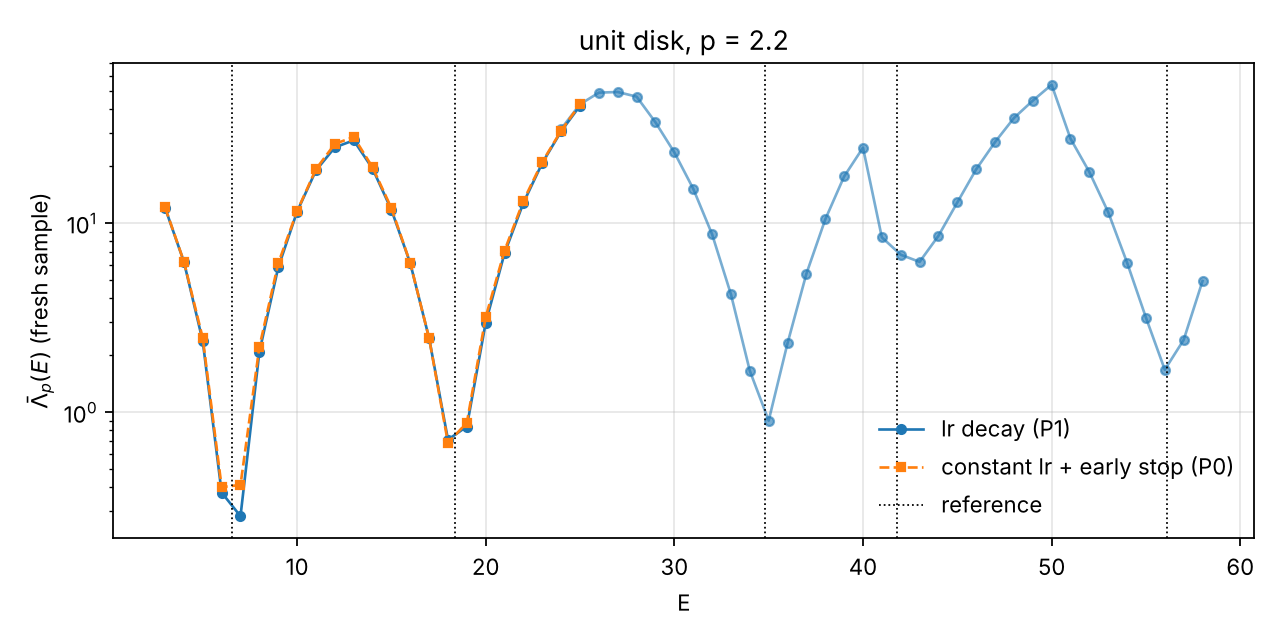
\includegraphics[width=.325\textwidth]{plap_disk_curves.png}
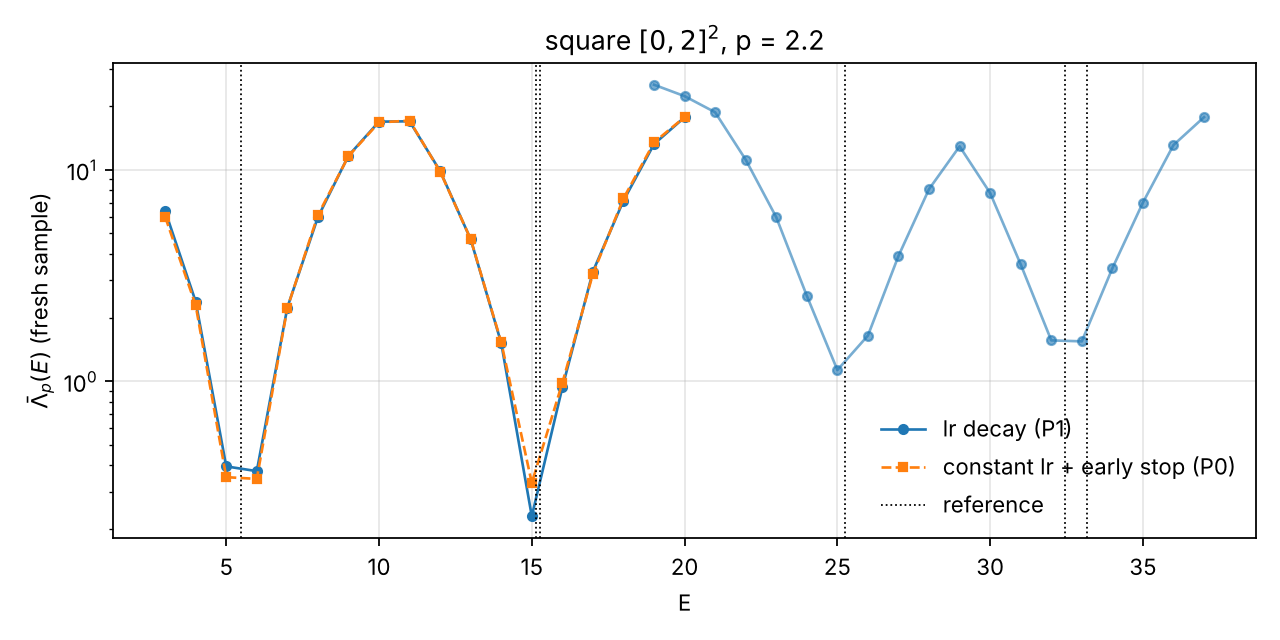
\includegraphics[width=.325\textwidth]{plap_square_curves.png}
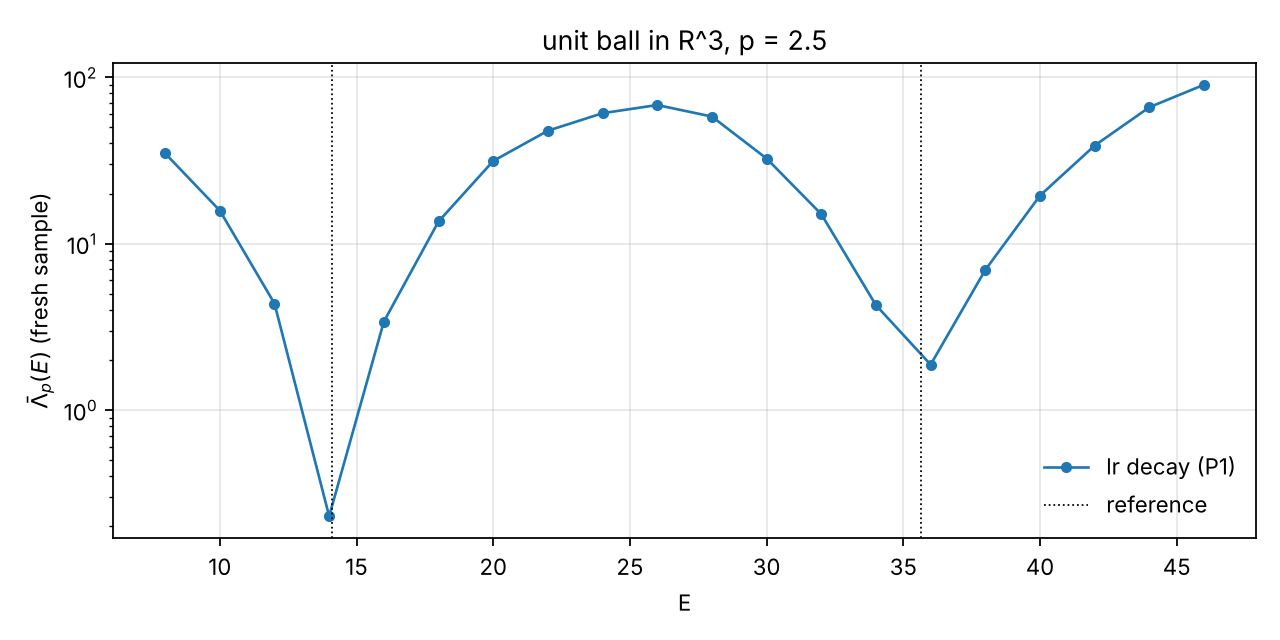
\includegraphics[width=.325\textwidth]{plap_ball_curves.png}
\caption{Loss curves $\bar\Lambda_p(E)$ (fresh sample, logarithmic scale): unit disk, $p=2.2$ (left), square $[0,2]^2$, $p=2.2$ (centre), unit ball of $\R^3$, $p=2.5$ (right). Dotted lines: reference eigenvalues. P1: learning-rate decay; P0: constant learning rate with early stopping.}
\label{fig.plap}
\end{figure}

\begin{table}[tbp]
\centering\small
\caption{Seed dependence for $p=2.2$ (seeds 0, 1, 2; local three-node windows, $h=0.5$, settings of Table~\ref{tab.plap}). For the second eigenvalue of the square the close eigenvalues $15.1429$ (diagonal nodal line) and $15.2808$ (midline) lie in the same minimum of the loss curve; each seed converges to one of them, no mean is given, and the difference is measured to the nearer one.}
\label{tab.plap.seeds}
\setlength{\tabcolsep}{4pt}
\begin{tabular}{lcccccc}
\toprule
eigenvalue & $E_{\rm ref}$ & $E_{\rm PINN}$ (seeds 0, 1, 2) & mean & spread & max.\ rel.\ diff.\ (\%) & $E_{\rm curve}$ (seeds 0, 1, 2)\\
\midrule
disk $E_1$ & 6.5317 & 6.5320, 6.5329, 6.5285 & 6.5311 & 0.0044 & 0.05 & 6.54, 6.54, 6.54\\
disk $E_2$ & 18.3929 & 18.4069, 18.3890, 18.3968 & 18.3976 & 0.0179 & 0.08 & 18.41, 18.45, 18.46\\
square $E_1$ & 5.4950 & 5.4902, 5.4867, 5.4966 & 5.4912 & 0.0100 & 0.15 & 5.52, 5.49, 5.41\\
square $E_2$ & 15.1429 / 15.2808 & 15.1440, 15.2467, 15.1396 & -- & -- & 0.22 & 15.16, 15.51, 15.42\\
\bottomrule
\end{tabular}
\end{table}

Table~\ref{tab.plap} and Fig.~\ref{fig.plap} show that the first and second eigenvalues agree with
the references to within $0.1\%$ in the three domains. Beyond them, the same scan detects further
eigenvalues: in the disk, the third to fifth minima match the eigenvalues with two nodal diameters,
one nodal circle and three nodal diameters, and in the square the third and fourth minima match the
$2\times2$ cell mode and the mode with both diagonals as nodal lines, with relative differences
below $0.1\%$ except for the radial mode with a nodal circle ($+0.41\%$; its gradient vanishes on a
whole circle, which gives the largest residual floor). For the ball of $\R^3$ the shooting value
$14.1112$ and the axisymmetric finite element value $35.6315$ are matched to $0.08\%$ and $0.01\%$.
The rows $k\ge3$ and the ball are single runs; with three seeds the first two eigenvalues of the disk
and of the square have a spread of $E_{\rm PINN}$ of $0.004$--$0.018$ and a largest relative difference of
$0.15\%$ (Table~\ref{tab.plap.seeds}). Two caveats apply. Close eigenvalues are not separated: in the
square, $15.1429$ (diagonal nodal line) and $15.2808$ (midline nodal line) give a single minimum and the
seed decides which one the network converges to; the same happens for $32.46$ and $33.17$. And the
reference $35.63$ is an eigenvalue of the ball with one nodal plane and an upper bound for the second
eigenvalue; that it is the second eigenvalue is not proved.

\emph{Error sources and range of $p$.} The convergence study of Appendix~\ref{app.conv} identifies two
dominant error sources of the \emph{curve}: optimization noise (with a constant learning rate the vertex
of the curve has errors up to $2\%$; a decaying learning rate reduces them to $0.2\%$) and a residual
floor at the critical points of the eigenfunction, where a smooth network cannot satisfy the equation
for $p>2$ (Lemma~\ref{lem.critical}); this floor biases the minimum of the curve by $+0.2$ to $+0.8\%$ and
is not removed by larger networks, more points or longer training. The refined value $E_{\rm PINN}$ is
insensitive to all these settings (at most $0.05\%$ for every configuration with learning-rate decay,
$\ge1500$ epochs and $N\ge5000$). Hence the loss curve should be used to \emph{detect} the eigenvalues and
the frozen-network quotient to \emph{compute} them. The floor grows with $p$: the method is validated
for $p\in[2.2,3]$ (and $p=2.5$ in three dimensions), and $p=4$ is marginal (Table~\ref{tab.plap.p}). For
$p=1.5$ the strong form fails (no minimum near $E_1$); replacing $\Delta_p$ by the regularized operator
$\operatorname{div}((|\nabla u|^2+\nu^2)^{(p-2)/2}\nabla u)$ cures the failure, with a difference of
$-0.31\%$ to $E_1$ for $\nu=0.03$ in a single-seed test (Table~\ref{tab.plap.reg}).

% ===========================================================================
\section{Cost and practical aspects}\label{sec.cost}

One epoch of the scan needs $\Delta u_\theta$, so its cost is linear in $d$; a scan costs (number of
nodes) $\times$ (cost of one training), and by Proposition~\ref{prop.stability} the grid only needs to
separate the eigenvalues, since the accuracy comes from the Rayleigh quotient and not from $h$ (cost
model in Appendix~\ref{app.cost}). Table~\ref{table.cost} compares the scan with a Rayleigh-quotient PINN
with deflation \cite{Rowan-Evans-Maute-Dootsan,Holliday-Lindner-Ditto,E-Yu} on the unit square, with the
same network, boundary factor and sample size, on one CPU thread and three seeds. For the lowest
eigenvalues of a two-dimensional problem deflation is \emph{cheaper}: the 18-node scan is $2.6$ times
slower than deflation without early stopping and $8.4$ times slower than deflation with early stopping;
and deflation \emph{resolves multiplicities}, which the scan does not. The scan was more accurate in
these runs ($4\times10^{-5}$ against $2.3\times10^{-3}$ and $3.1\times10^{-2}$); we did not push the
training of the deflation baseline further, so the cost of deflation at equal accuracy was not
measured, and we compared only $K=6$. The advantages of the scan lie elsewhere: (i) sub-windows are
independent and can be computed in parallel, whereas deflation is sequential; (ii) each eigenvalue
carries its own a posteriori enclosure, computed from its own network and independent of the accuracy of
other eigenpairs; (iii) no orthogonalization against lower eigenfunctions is needed, so errors do not
accumulate with the index (for deflation the number of lower eigenvalues grows like $E^{d/2}$ by Weyl's
law), although the scan still has to reach a high window by continuation, since cold starts are
unreliable; (iv) the scan applies verbatim to nonlinear problems such as the $p$-Laplacian.

\begin{table}[tbp]
\centering\small
\caption{Cost on the unit square (one CPU thread, $3\times128$ network, 5000 points per epoch, shared machine: times indicative). Mean [min, max] over seeds 0, 1, 2 unless stated. The six lowest eigenvalues counted with multiplicity are $2\pi^2$, $5\pi^2$ (double), $8\pi^2$, $10\pi^2$ (double). Refinement times in parentheses.}
\label{table.cost}
\begin{tabular}{lrll}
\toprule
method & wall time (s) & eigenvalues obtained & max.\ rel.\ error\\
\midrule
deflation, $K=6$, early stopping & 247 [229, 262] & 6 (with mult.) & $3.1\times10^{-2}$\\
deflation, $K=6$, no early stopping & 813 [796, 830] & 6 (with mult.) & $2.3\times10^{-3}$\\
scan $[17.3,102.3]$, 18 nodes & 2082 [2023, 2135] (+77--110) & 4 distinct & $4.1\times10^{-5}$\\
scan $[0,105]$, 80 nodes (Table~\ref{table.1}; seed 0) & 6534 (+413) & 4 distinct & $3.5\times10^{-5}$\\
cold start $[95,102]$, 5 nodes, $\mu=5000$ & 818--1008 & $10\pi^2$ at 8/15 nodes & $2.1\times10^{-5}$ (one run)\\
\bottomrule
\end{tabular}
\end{table}

% ===========================================================================
\section{Conclusions}\label{sec.conclusions}

Eigenvalues of elliptic operators can be computed with neural networks as the zeros of a residual
loss curve, without the Rayleigh quotient and without orthogonality. For self-adjoint problems the
curve is the squared distance to the spectrum; the penalized loss used in practice has an explicit
loss curve without spurious local minima, which yields the rule $\mu\ge D^2$; the detection is stable
whenever the measured error level is small compared with the squared gaps; and, once a minimum is
detected, the Rayleigh quotient of the frozen network gives an accurate value with a Weinstein and
Kato--Temple enclosure. The method agrees with exact values in dimensions two to four and with independent finite element
computations in dimensions two and three (seed means within $0.1\%$ of FEM for the potentials), and is
feasible in dimension ten. Because the mechanism needs no orthogonality, it extends to the
$p$-Laplacian: the zeros of the loss curve are exactly the eigenvalues, and eigenvalues beyond the
second one are detected in a single scan and agree with independent references.

\emph{Limitations.} The scan does not resolve multiplicities or clusters closer than the error level,
and it can miss an eigenvalue when the warm-started network stays on a neighbouring branch; training
from scratch at a high $E$ is unreliable; for the lowest eigenvalues of linear problems deflation is
cheaper, and finite elements are much cheaper and more accurate in dimensions two and three; no bound
on the training error is proved; for the $p$-Laplacian there is no a posteriori certificate, the
accuracy degrades for $p\ge4$, and for $p<2$ the strong form requires a regularization, which changes
the eigenvalue slightly. A weak-form version of the loss is a natural direction for future work.

\clearpage
% ===========================================================================
\appendix

\section{Proofs}\label{app.proofs}
This appendix contains the proof of existence of minimizers of \eqref{Lambda} and the proofs of all the propositions of Sections~\ref{sec.approach} and \ref{sec.nolin}.

\subsection{Existence of minimizers}
We show that the minimization problem leading to the loss curve $\Lambda(E)$ in \eqref{Lambda} admits
a solution, in the case of the hard-wall potential \eqref{conf.V} with $\Omega\subset \R^{d}$ bounded.
(Given \eqref{cota.igual}, the existence also follows from the spectral decomposition, the minimizers
being the eigenfunctions of the eigenvalue(s) closest to $E$; the proof below does not use the spectral
theorem.) The natural space is $H^2(\Omega) \cap H^1_0(\Omega)$.

\begin{theorem}\label{teo.min}
Let $V(x)$ be as in \eqref{conf.V} with $\Omega\subset \R^{d}$ bounded and either convex or of class $C^{1,1}$. Given $E\in\R$, there exists $u_E\in H^2(\Omega)\cap H^1_0(\Omega)$ such that
$$
\Lambda(E) = \Lambda(u_E, E) = \inf_{u\in H^2(\Omega)\cap H^1_0(\Omega)\setminus\{0\}}\Lambda(u, E),
$$
where $\Lambda(u, E)$ is given in \eqref{Lambda}.
\end{theorem}

\begin{proof}
The result follows from the \emph{direct method in the Calculus of Variations}. Fix $E\in\R$, and consider a minimizing sequence $\{u_j\}_{j \in \N} \subset H^2(\Omega) \cap H^1_0(\Omega)$ such that $\|u_j\|_2 = 1$ and
$
\Lambda(E) = \lim_{j \to \infty} \Lambda(u_j, E).
$
In particular,
\begin{equation}\label{cota.Lambda}
0 \le \Lambda(u_j, E) \le C,
\end{equation}
for some constant $C > 0$. Now observe that
\begin{align*}
\Lambda(u_j, E) &= \int_\Omega (\Delta u_j + Eu_j)^2\, dx = \int_\Omega (\Delta u_j)^2\, dx + 2E\int_\Omega u_j \Delta u_j \, dx+ E^2.
\end{align*}
If $E=0$ there is nothing to do. Otherwise, using the inequality $ab\le \theta a^2 + \frac{b^2}{4\theta}$ for any $a, b\ge0$ and $\theta >0$ we estimate
$$
\int_\Omega |u_j| |\Delta u_j|\, dx \le \theta \int_\Omega (\Delta u_j)^2\, dx + \frac{1}{4\theta}\int_\Omega u_j^2\, dx.
$$
Taking $\theta=1/(4|E|)$, we obtain $2|E|\int_\Omega|u_j||\Delta u_j|\,dx\le\frac12\int_\Omega(\Delta u_j)^2\,dx+2E^2$, and therefore
\begin{equation}\label{cota.Lambda2}
\Lambda(u_j, E)\ge \frac12 \int_\Omega (\Delta u_j)^2\, dx -E^2.
\end{equation}
Combining \eqref{cota.Lambda}, \eqref{cota.Lambda2} we get $\|\Delta u_j\|_2^2\le2(C+E^2)$. Since $\Omega$ is convex or of class $C^{1,1}$, $\|u\|_{H^2(\Omega)}\le C_\Omega\|\Delta u\|_2$ for $u\in H^2(\Omega)\cap H^1_0(\Omega)$, so the sequence $\{u_j\}_{j\in\N}$ is bounded in $H^2(\Omega)\cap H^1_0(\Omega)$.
Therefore, up to a subsequence, $u_j \rightharpoonup u_E$ weakly in $H^2(\Omega) \cap H^1_0(\Omega)$.
Since the functional
$
u \mapsto \int_\Omega (\Delta u + E u)^2\, dx
$
is convex, it is weakly lower semicontinuous, so
$$
\int_\Omega (\Delta u_E + E u_E)^2\, dx \le \liminf_{j \to \infty} \int_\Omega (\Delta u_j + E u_j)^2\, dx.
$$
Moreover, the embedding $H^2(\Omega)\cap H^1_0(\Omega)\hookrightarrow L^2(\Omega)$ is compact, so
$\int_\Omega u_E^2\, dx = \lim_{j\to\infty} \int_\Omega u_j^2\, dx = 1$.
Hence, $u_E$ is admissible and attains the minimum.
\end{proof}

\subsection{Proofs of the propositions}
Throughout, $L$, $u_k$, $E_k$, $\ell(E)$ are as in Section~\ref{sec.approach} and $\|\cdot\|=\|\cdot\|_2$.

\begin{proof}[Proof of Proposition~\ref{prop.penalized}]
Write $u=\sum_ka_ku_k$, $s=\|u\|^2$. Then $\|(L-E)u\|^2=\sum_k(E_k-E)^2a_k^2\ge \ell^2s$, with equality
iff $u\in N_E$, the span of the eigenfunctions with $|E_k-E|=\ell$. Hence
$\bar\Lambda(u,E)\ge g(s):=\ell^2s+\mu(s-1)^2$, with equality iff $u\in N_E$. If $\ell^2<2\mu$, $g$ attains its
minimum on $[0,\infty)$ only at $s_*=1-\ell^2/(2\mu)$, with $g(s_*)=\ell^2-\ell^4/(4\mu)$; if $\ell^2\ge2\mu$, $g$ is
increasing and its minimum is $g(0)=\mu$. This gives the formula and the minimizers; the residual term
at the minimizer is $\ell^2s_*$. For the critical points, the derivative of $\bar\Lambda(\cdot,E)$ at $u$ in
the direction $u_k$ is $2[(E_k-E)^2-2\mu(1-s)]a_k$, so $u\ne0$ is critical iff all $k$ with
$a_k\ne0$ share the same $\lambda=(E_k-E)^2$ and $s=1-\lambda/(2\mu)$ (thus $\lambda<2\mu$). If
$\lambda>\ell^2$ and $u_j$ is an eigenfunction with $|E_j-E|=\ell$, then $a_j=0$ and
$\bar\Lambda(u+tu_j,E)=\bar\Lambda(u,E)+t^2(\ell^2-\lambda)+\mu t^4$, which is smaller for small $t\ne0$; so
$u$ is a saddle. Likewise $\bar\Lambda(tu_j,E)=\mu+t^2(\ell^2-2\mu)+\mu t^4$, so $u=0$ is not a local
minimizer if $\ell^2<2\mu$. The critical points with $\lambda=\ell^2$ are the global minimizers.
\end{proof}

\begin{proof}[Proof of Corollary~\ref{cor.mu}]
This follows directly from Proposition~\ref{prop.penalized}, since $\mathcal R_\mu=\psi(\ell^2)$ with
$\psi(t)=t(1-t/(2\mu))_+$, which increases on $[0,\mu]$, decreases on $[\mu,2\mu]$ and vanishes for
$t\ge2\mu$. The location of the minima does not depend on $\mu$, and the normalized quotient
$\Lambda(u_E,E)=\ell(E)^2$ is independent of $\mu$.
\end{proof}

\begin{proof}[Proof of Proposition~\ref{prop.rayleigh}]
Assume $\|u\|=1$, $u=\sum_ja_ju_j$, $\rho=\rho(u)$, $\eta=\eta(u)$. (a) follows from
$\|(L-E)u\|^2=\|(L-\rho)u\|^2+(\rho-E)^2$, since $\langle(L-\rho)u,u\rangle=0$. (b) $\|(L-E)u\|^2=
\sum_j(E_j-E)^2a_j^2\ge \ell(E)^2$. (c) Let $\beta=\rho+\gamma$. Since $\sigma\cap(E_k,\beta)=\emptyset$,
$(E_j-E_k)(E_j-\beta)\ge0$ for all $j$; expanding around $\rho$ and using $\sum a_j^2=1$,
$\sum a_j^2(E_j-\rho)=0$, $\sum a_j^2(E_j-\rho)^2=\eta^2$ gives $0\le\eta^2+(\rho-E_k)(\rho-\beta)$, i.e.\
$\rho-E_k\le\eta^2/\gamma$. The lower bound follows in the same way with $\alpha=\rho-\gamma$.
\end{proof}

\begin{proof}[Proof of Proposition~\ref{prop.stability}]
Write $\ell_i=\ell(E^i)$. (a) $\ell_i^2\le\tilde\Lambda_i+\delta\le\epsilon+\delta$. (b) Some node satisfies
$|E^i-E_k|\le h/2$, and then $\tilde\Lambda_i\le \ell_i^2+\delta\le h^2/4+\delta$. (c) Let $E_k$ be the
eigenvalue with $|E^m-E_k|=\ell_m$ and assume $\ell_m\ge h$. The neighbour $E^{m'}$ on the side of $E_k$ has
$\ell_{m'}\le \ell_m-h$, so $\ell_m^2-\delta\le\tilde\Lambda_m\le\tilde\Lambda_{m'}\le(\ell_m-h)^2+\delta$, i.e.\
$2h\ell_m\le h^2+2\delta$. (d) Let $I=[E_k-\tau-h,E_k+\tau+h]$ and let $E^m$ minimize $\tilde\Lambda$ over
the nodes in $I$, and $\gamma_k=\dist(E_k,\sigma\setminus\{E_k\})$. By (b), $\tilde\Lambda_m\le h^2/4+\delta$, hence $\ell_m\le\tau$. If the eigenvalue closest
to $E^m$ were $E_j\ne E_k$, then $|E^m-E_k|\ge\gamma_k-\tau>\tau+h$, contradicting $E^m\in I$; hence
$|E^m-E_k|\le\tau$, both neighbours of $E^m$ lie in $I$, and $E^m$ is a discrete local minimum.
\end{proof}

\begin{proof}[Proof of Proposition~\ref{prop.plap}]
(a) Since $\Delta_pu_k=-E_k|u_k|^{p-2}u_k$, the residual is $(E-E_k)|u_k|^{p-2}u_k$ and the penalty
vanishes. (b) If $E\in\sigma_p$, $\Lambda_p(E)=0$ by (a). Conversely, by the homogeneity
$\Delta_p(tu)=|t|^{p-2}t\Delta_pu$, every $u\ne0$ can be written as $tw$ with $\|w\|_p=1$, and
$\bar\Lambda_p(tw,E)=t^{2(p-1)}Q(w)+\mu(t^p-1)^2$ with $Q(w)=\int(\Delta_pw+E|w|^{p-2}w)^2$; hence
$\Lambda_p(E)=0$ forces $\inf_{\|w\|_p=1}Q(w)=0$. Take $w_n$ with $\|w_n\|_p=1$ and
$f_n:=-\Delta_pw_n-E|w_n|^{p-2}w_n\to0$ in $L^2$. Testing with $w_n$ and using
$\|w\|_2\le C_S\|\nabla w\|_p$ (here $p\ge2d/(d+2)$ is used),
$\|\nabla w_n\|_p^p\le E+C_S\|f_n\|_2\|\nabla w_n\|_p$, so $w_n$ is bounded in $W^{1,p}_0$. Up to a
subsequence $w_n\rightharpoonup w$ in $W^{1,p}_0$ and $w_n\to w$ in $L^p$, so $\|w\|_p=1$ and
$|w_n|^{p-2}w_n\to|w|^{p-2}w$ in $L^{p'}\subset W^{-1,p'}$; also $f_n\to0$ in $W^{-1,p'}$. Thus
$-\Delta_pw_n\to E|w|^{p-2}w$ in $W^{-1,p'}$, and by continuity of $(-\Delta_p)^{-1}\colon
W^{-1,p'}\to W^{1,p}_0$, $w_n\to w$ strongly, with $-\Delta_pw=E|w|^{p-2}w$, $w\ne0$.
\end{proof}

\begin{proof}[Proof of Proposition~\ref{prop.ck}]
Write $u=u_k$ and $q=2(p-1)$. Testing the weak form of \eqref{p-eigen} with $u$ gives
$\|\nabla u\|_p^p=E_k\|u\|_p^p=E_k$. (b) is $\|u\|_2=1$.

(a) Let $1<p<2$, so that $0<q<p$. H\"older's inequality with exponents $p/q$ and $p/(p-q)$ gives
$c_k=\int_\Omega|u|^q\le|\Omega|^{1-q/p}\big(\int_\Omega|u|^p\big)^{q/p}=|\Omega|^{(2-p)/p}$, since
$1-q/p=(2-p)/p$. For the lower bound note that $p<2\le d$, so $p^*$ is defined and $q<p<p^*$. Writing
$|u|^p=|u|^{p\theta}|u|^{p(1-\theta)}$ and applying H\"older's inequality with exponents
$q/(p\theta)$ and $p^*/(p(1-\theta))$, whose reciprocals add up to $1$ by the definition of $\theta$, we
obtain the interpolation inequality
\[
1=\|u\|_p\le\|u\|_q^{\theta}\|u\|_{p^*}^{1-\theta}\le c_k^{\theta/q}\big(S_*\|\nabla u\|_p\big)^{1-\theta}
=c_k^{\theta/q}\big(S_*E_k^{1/p}\big)^{1-\theta}.
\]
Raising to the power $q/\theta$ gives $c_k\ge S_*^{-q(1-\theta)/\theta}E_k^{-q(1-\theta)/(p\theta)}$.

(c) Let $p>2$, so that $q>p$. H\"older's inequality with exponents $q/p$ and $q/(q-p)$ gives
$1=\int_\Omega|u|^p\le|\Omega|^{1-p/q}c_k^{p/q}$, i.e.\ $c_k\ge|\Omega|^{-(q-p)/p}=|\Omega|^{(2-p)/p}$, since
$q-p=p-2$. For the upper bound we need $W^{1,p}_0(\Omega)\hookrightarrow L^q(\Omega)$. If $p>d$ this follows
from Morrey's embedding into $L^\infty(\Omega)$ and the boundedness of $\Omega$; if $p=d$,
$W^{1,d}_0(\Omega)$ embeds into $L^s(\Omega)$ for every $s<\infty$; if $p<d$, the Sobolev embedding into
$L^{p^*}(\Omega)$ and H\"older's inequality give the embedding when $q\le p^*$, and
$q\le p^*\iff2(p-1)(d-p)\le dp\iff d(p-2)\le2p(p-1)$. Then
$c_k=\|u\|_q^q\le S_q^q\|\nabla u\|_p^q=S_q^qE_k^{q/p}$. Finally, writing $p=2+t$ with $t>0$,
$\frac{2p(p-1)}{p-2}=2\big(t+3+\frac2t\big)\ge6+4\sqrt2>11$, so the condition holds for all $p>2$ when
$d\le11$.
\end{proof}

The constant $S_*$ in Proposition~\ref{prop.ck} depends only on $d$ and $p$, whereas $S_q$ depends in
general on $\Omega$ (in particular when $p\ge d$). For $1<p<2$ the curvature of the bounding parabolas
is bounded above uniformly in $k$ but may decrease as $k$ grows, while for $p>2$ it is bounded below
uniformly but the upper bound grows like $E_k^{2(p-1)/p}$.

% ---------------------------------------------------------------------------
\section{Implementation details}\label{sec.implementation}
This appendix describes the network, the training protocol and the settings of every linear example, and the cost model behind Section~\ref{sec.cost}.

\subsection{Network and boundary factor}
We use a fully connected feed-forward multilayer perceptron with three hidden layers of 128 neurons
and $\tanh$ activations (Fig.~\ref{NN.fig}), mapping $x\in \R^d$ to $\text{NN}(x) \in \mathbb{R}$. All
linear layers are initialized with Xavier uniform initialization with the gain for $\tanh$, and all
biases are set to zero. The homogeneous Dirichlet condition is enforced by a boundary factor $B$ with
$B=0$ on $\partial\Omega$ and $B>0$ in $\Omega$; the network returns $u(x)=B(x)\,\text{NN}(x)$. The factors
used are smooth, vanish exactly on $\partial\Omega$ and are comparable to the distance to the boundary:
\[
\begin{array}{ll}
\text{Domain} & B(x)\\ \hline
\text{Ball } \{|x|<1\}\subset\R^d,\ d=2,3,4 & 1-|x|^2\\
\text{Square } (0,a)^2,\ a=1,2 & x_1(a-x_1)\,x_2(a-x_2)\\
\text{Triangle with vertices } (0,0),(1,0),(0,1) & x_1x_2(1-x_1-x_2)\\
\text{Annulus } \{\tfrac12<|x|<1\} & (|x|-\tfrac12)(1-|x|)
\end{array}
\]
(and $1-|x|^2$ also for the ball of $\R^{10}$). Since $u=B\,\mathrm{NN}$ satisfies the boundary
condition exactly and is smooth, every network function belongs to $\mathrm{Dom}(L)$; this is what
makes the a posteriori bounds of Section~\ref{sec.certificate} applicable to the trained networks.

\begin{figure}[H]
\centering
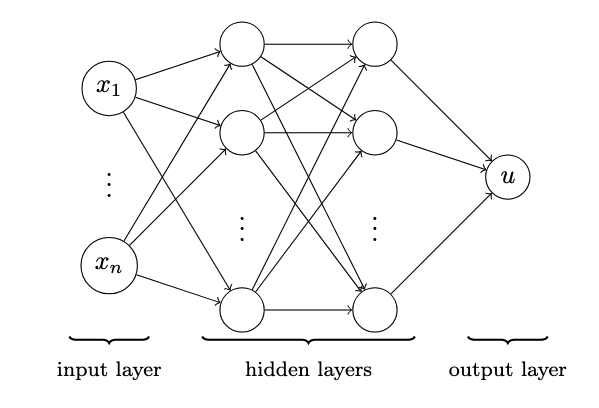
\includegraphics[width=.35\columnwidth]{NN-Tikz.png}
\caption{A fully connected feedforward NN with a $d$-dimensional input and a 1-dimensional output.}
\label{NN.fig}
\end{figure}

The hard-wall potential
\begin{equation}\label{conf.V}
V(x) = \begin{cases}
0 & \text{if } x\in \Omega\\
\infty & \text{if } x\not\in \Omega
\end{cases}
\end{equation}
is equivalent to the Dirichlet problem \eqref{eigen2}. In all the examples with a potential the problem
is also posed in a bounded domain with the Dirichlet condition.

\subsection{Training and detection}
All integrals are approximated by Monte Carlo; in the code they are replaced by sample means, i.e.\ by
integrals with respect to $dx/|\Omega|$, and all statements are invariant under this change of measure.
The parameters are optimized with Adam, constant learning rate $10^{-3}$, and at most $N_{\rm ep}$ Adam
steps (epochs) per node; at each epoch a fresh sample of $N$ points ($N=5000$ unless stated) is drawn.
Training at a node stops early if the loss does not decrease by $\mathrm{tol}=10^{-5}$ in 300
consecutive epochs. For each $E^i$ the network is initialized with the weights obtained at $E^{i-1}$
(warm start); in some scans it is re-initialized every 15--60 grid points. Upon completion we obtain
the discrete loss curve $\bar \Lambda(E^i)=\bar\Lambda(u^i, E^i)$, and each local minimum below a threshold
$\epsilon>0$ is taken as an approximate eigenvalue. The threshold was chosen per example after
inspecting the curve; Proposition~\ref{prop.stability} shows what any choice guarantees, and the
certificate of Section~\ref{sec.certificate} makes the threshold unnecessary for accepting a detection.
In the tables, $\mathrm{Residual}=\frac1N\sum_{i=1}^N(\Delta u-Vu+Eu)^2(x_i)$ is the first term of
\eqref{lossmu}; since $\frac1N\sum u(x_i)^2\approx1$ at the minima, $\mathrm{Residual}\approx\Lambda(u,E)=r^2$.
The window, the grid step, $\mu$, $N_{\rm ep}$, the type of start and the number of seeds of every
example are listed in Table~\ref{table.settings}, together with the regime of $\mu$ with respect to
Corollary~\ref{cor.mu}.

\begin{table}[H]
\centering\scriptsize
\caption{Settings of the linear examples ($3\times128$ network, Adam with learning rate $10^{-3}$,
early stopping 300/$10^{-5}$). $h$: grid step; $N_{\rm ep}$: maximal number of epochs per node;
start: warm (continuation from the previous node), cold (fresh network), re-init.\ (fresh network
every $n$ nodes); $D=\max\ell(E)$ over the window (Corollary~\ref{cor.mu}); regime: (ii) faithful
($\mu\ge D^2$), (iii) $\frac12D^2\le\mu<D^2$, (iv) collapse possible ($\mu<\frac12D^2$), see
Corollary~\ref{cor.mu}. Single runs unless the number of seeds is given (seed 0 where the seed was
recorded). $^a$Window and step of the accompanying notebook (approximate for the full-scan curves of
Figs.~\ref{lossNN.fig}, \ref{loss3D.fig}, \ref{pot2.fig}--\ref{fig.well-two}). $^b$Reduced network $3\times64$, $N=3000$.}
\label{table.settings}
\begin{tabular}{@{}llccccll@{}}
\toprule
example & window & $h$ & $\mu$ & $N_{\rm ep}$ & start, seeds & $D^2$ & regime\\
\midrule
disk (Fig.~\ref{lossNN.fig}) & $[0,32]^a$ & -- & 100 & 3000 & warm & 33.4 & (ii)\\
square (Fig.~\ref{eigen55.fig}) & $[44,55]$ & -- & 3000 & -- & cold/warm & 31.9 & (ii)\\
square (Tab.~\ref{table.1}) & $[0,105]$ & 1.33 & 500 & 5000 & re-init.\ 25 & 390 & (ii)$^\ast$\\
square (App.~\ref{sec.analysis}, \S\ref{sec.cost}) & $[15,55]$, $[17.3,102.3]$ & 5 & 450 & 3000 & warm, 3 seeds & 219 & (ii)\\
square ($\mu$ study) & $[40,60]$, $[15.6,53.1]$ & 2, 2.5 & 1--$10^4$ & $2000^b$ & warm, 2 seeds & 114, 219 & all\\
square (cold start) & $[95,102]$ & 1.75 & 450--$2\cdot10^4$ & 5000 & cold, 1--3 seeds & -- & --\\
ball $\R^3$ (Fig.~\ref{loss3D.fig}) & $[0,70]^a$ & -- & 100 & 2000 & re-init.\ 15 & 97.4 & (ii)\\
ball $\R^4$ (Fig.~\ref{loss3D.fig}) & $[0,55]^a$ & -- & 200 & 2000 & warm & 216 & (iii)\\
triangle (Fig.~\ref{loss.lap.triang.fig}), $N\!=\!4000$ & $[0,180]$ & 1.8$^a$ & 15000 & 2000 & re-init.\ 50$^a$ & 2435 & (ii)\\
Tabs.~\ref{table.2}, \ref{table.4} & 3 nodes/eigenv. & 1 & as above & 2000 & cold/warm & $\le1.2$ & (ii)\\
$\omega=1$ (Fig.~\ref{pot2.fig}) & $[0,55]^a$ & 0.7 & 100 & 3000 & re-init.\ 50 & 34.7 & (ii)\\
$\omega=10$ (Fig.~\ref{pot1.fig}) & $[0,55]^a$ & 0.7 & 100 & 3000 & re-init.\ 50 & 204 & (iv)\\
wells (Fig.~\ref{fig.well-two}) & $[0,75]^a$ & 0.63 & 400/1000 & 2000 & re-init.\ 50 & 92/97 & (ii)\\
FEM windows (Tab.~\ref{table.fem}) & $4\times7$ nodes & 0.5 & 400/1000/100 & 2000/3000 & cold/warm, 2--3 seeds & $\le 2.3$ & (ii)\\
blind scan (Tab.~\ref{table.blind}) & $[4.7,49.7]$ & 1.5 & 400 & 2000 & warm & 41.1 & (ii)\\
ball $\R^{10}$ (\S\ref{sec.d10}) & $[54,84]$ & 3 & 2000 & 2000 & warm & 93.7 & (ii)\\
\bottomrule
\multicolumn{8}{@{}l}{$^\ast$The re-initializations at $E\approx33,66,100$ are cold starts with $\mu\ll E^2/2$; branch switch and collapse were observed there (Appendix~\ref{sec.analysis}).}
\end{tabular}
\end{table}

\subsection{Cost model}\label{app.cost}
Let $W$ be the number of network parameters, $N$ the number of sampling points and $d$ the dimension.
The loss \eqref{lossmu} needs $\Delta u_\theta$, i.e.\ one backward pass for $\nabla u_\theta$ and $d$ further
passes for the diagonal of the Hessian, so one epoch costs $c_{\rm ep}=\kappa(d+2)NW$, linear in $d$
(we measured about $60+50d$ ms per epoch for the $3\times128$ network with 5000 points on one thread). If
$n_i$ epochs are used at node $E^i$, the scan of a window with $J$ nodes costs
\begin{equation}\label{cost.scan}
C_{\rm scan}=c_{\rm ep}\sum_{i=1}^Jn_i\le\kappa(d+2)NWJN_{\rm ep}.
\end{equation}
By Proposition~\ref{prop.stability} the grid only needs to separate the eigenvalues, $h\lesssim
\gamma_{\min}/2$, since the accuracy comes from the Rayleigh quotient and not from $h$; hence
$J\approx2(E^*-E_*)/\gamma_{\min}$. With warm start most nodes need few epochs (in the scan of
Table~\ref{table.1}, $302$--$3060$ epochs per node, median $\approx500$, against a maximum of $5000$). The
trainings in different sub-windows, each with its own warm start, are independent, so the wall-clock
time can be divided by the number of processors. A Rayleigh-quotient PINN with deflation
\cite{Rowan-Evans-Maute-Dootsan,Holliday-Lindner-Ditto,E-Yu} computes the $k$-th eigenpair by minimizing
$R(u)$ plus penalties for the overlap with the $k-1$ previous networks; an epoch needs only first
derivatives (cost $\kappa'NW$) plus the evaluation of the previous networks, so the first $K$ eigenpairs
cost $\approx\bar n\,NW(\kappa'K+\frac{\kappa_0}2K^2)$, sequentially, and errors in the computed
eigenfunctions bias all subsequent eigenvalues downwards (Courant--Fischer).

\emph{Setting of Table~\ref{table.cost}.} Both approaches use the same network, boundary factor and
sample size, on one CPU thread, with three seeds each. The deflation baseline minimizes $R(u)$ plus
$\beta\sum_{j<k}\langle u,u_j\rangle^2/(\|u\|^2\|u_j\|^2)$ with $\beta=200$, with or without early
stopping; the eigenvalue is its Rayleigh quotient. The scan uses a grid offset from the spectrum
($E=17.3,22.3,\dots,102.3$, $\mu=450$). In all three seeds of the offset scan, $2\pi^2$ appears at the
boundary node $E=17.3$ ($r^2\approx6.0$, against $6.6$--$6.8$ at $E=22.3$), not as an interior minimum, so
Proposition~\ref{prop.stability}(d) does not apply to it; it is identified through the Rayleigh quotient
at that node ($19.740$). The other three distinct eigenvalues are interior minima. The limitations of the
scan are: the cost of a full scan is (number of nodes) $\times$ (cost of one training), the second
derivatives make each epoch more expensive, and multiplicities and close clusters are not resolved
(Remark~\ref{rem.stability}).

% ---------------------------------------------------------------------------
\section{Further linear examples}\label{app.linear}
This appendix collects the linear examples not discussed in Section~\ref{sec.examples} and the details of the finite element validation.

\subsection{Disk and square}
Fig.~\ref{func.fig} shows the first four computed eigenfunctions in the unit disk (scan of
Fig.~\ref{lossNN.fig}, $\mu=100$). In the unit square we also computed the window $[44,55]$, which
contains one double eigenvalue $E_{(1,2)}=5\pi^2\approx49.348$, with $\mu=3000$ (Fig.~\ref{eigen55.fig}).
The loss curve of the scan of Table~\ref{table.1} is shown in Fig.~\ref{fig.collapse}
(Appendix~\ref{sec.analysis}) and the first two eigenfunctions in Fig.~\ref{loss.lap.square.fig.2}.
In all examples the windows start at or below the first eigenvalue, or the network is warm-started at
nodes close to the target; training from scratch at a high value of $E$ is unreliable
(Appendix~\ref{sec.analysis}).

\begin{figure}[H]
\centering
\begin{tabular}{cccc}
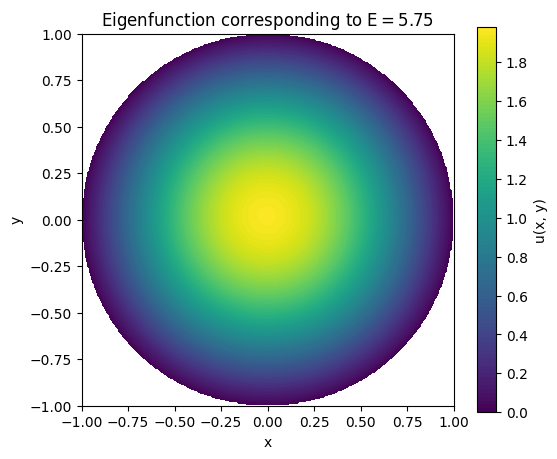
\includegraphics[width=.14\columnwidth]{eigen1-1.png} & 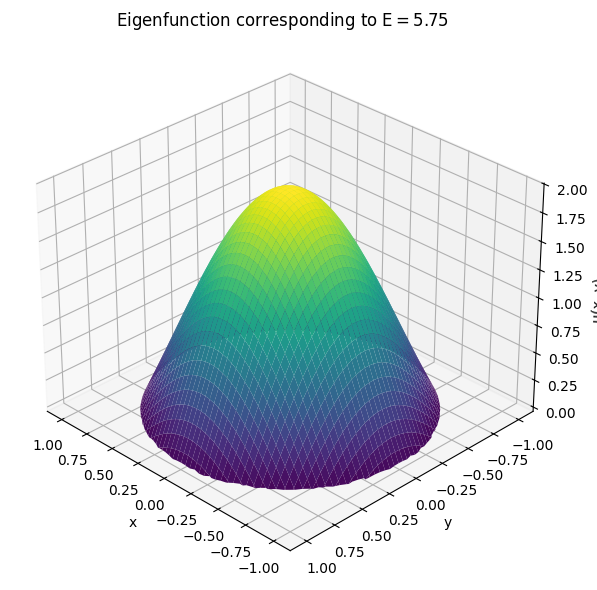
\includegraphics[width=.14\columnwidth]{eigen1-2.png} &
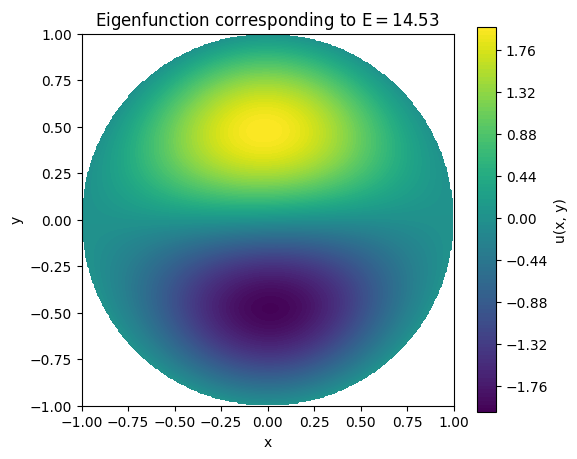
\includegraphics[width=.14\columnwidth]{eigen2-1.png} & 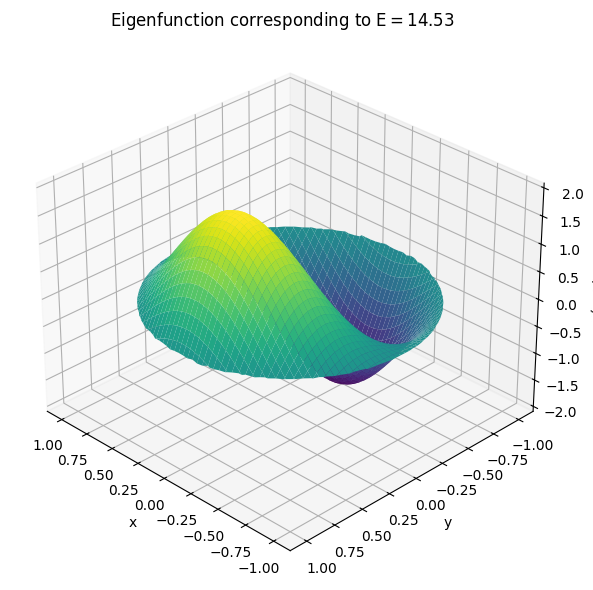
\includegraphics[width=.14\columnwidth]{eigen2-2.png} \\
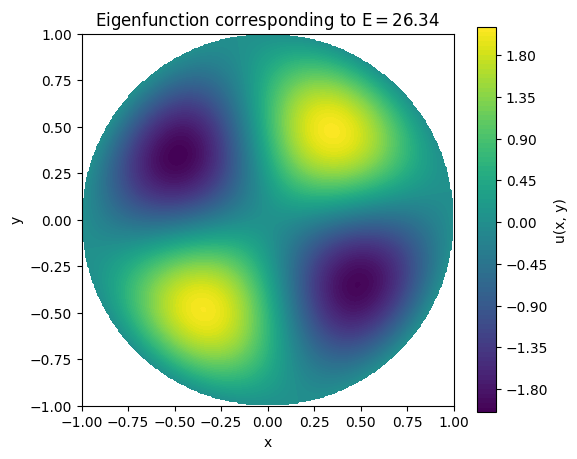
\includegraphics[width=.14\columnwidth]{eigen3-1.png} & 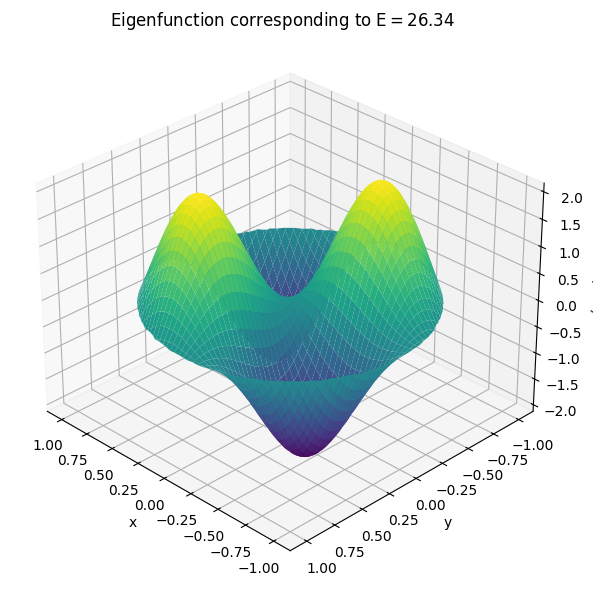
\includegraphics[width=.14\columnwidth]{eigen3-2.png} &
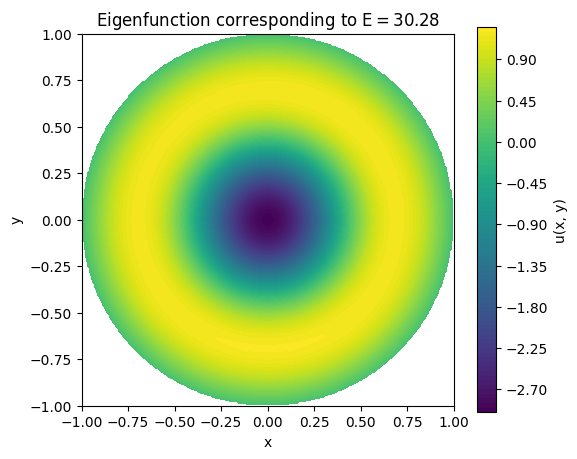
\includegraphics[width=.14\columnwidth]{eigen4-1.png} & 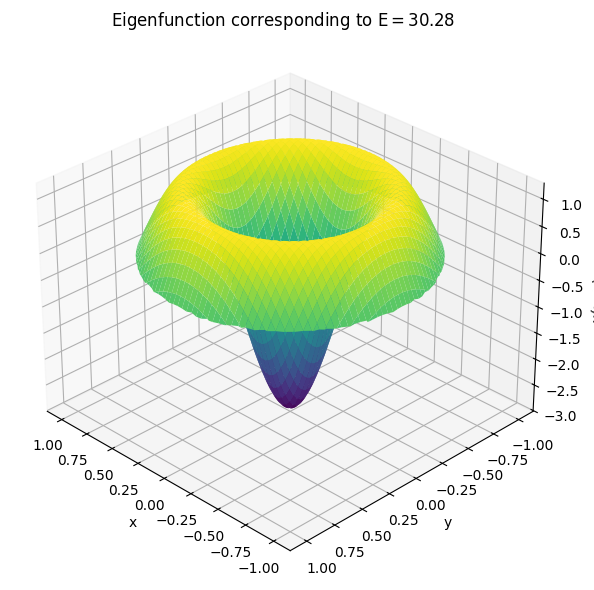
\includegraphics[width=.14\columnwidth]{eigen4-2.png} \\
\end{tabular}
\caption{The first four computed eigenfunctions of \eqref{eigen2} in the two-dimensional unit disk.}
\label{func.fig}
\end{figure}

\begin{figure}[H]
\centering
\begin{minipage}[t]{.4\textwidth}
\centering
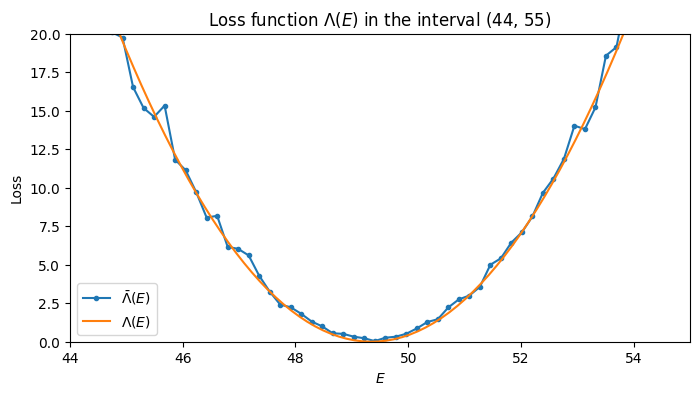
\includegraphics[width=\textwidth]{loss_2d_cuadrado_entre_45_y_55_1er_autovalor.png}
\caption{The loss curve $\bar\Lambda(E)$ in the unit square computed in the interval $[44,55]$, together
with the exact curve.}
\label{eigen55.fig}
\end{minipage}\hfill
\begin{minipage}[t]{.56\textwidth}
\centering
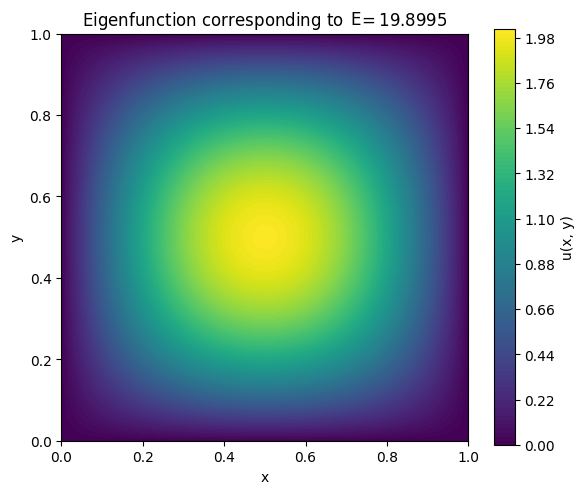
\includegraphics[width=.24\textwidth]{n=2_p=2_v=0_mu=150_cuadrado_autof1.png}
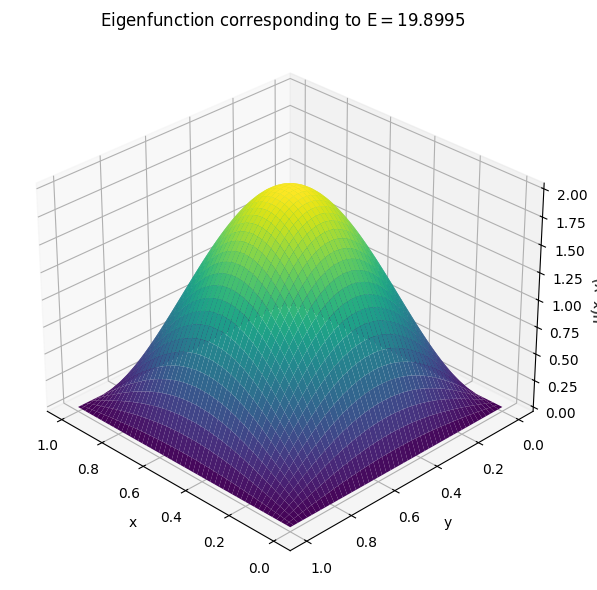
\includegraphics[width=.24\textwidth]{n=2_p=2_v=0_mu=150_cuadrado_autof13d.png}
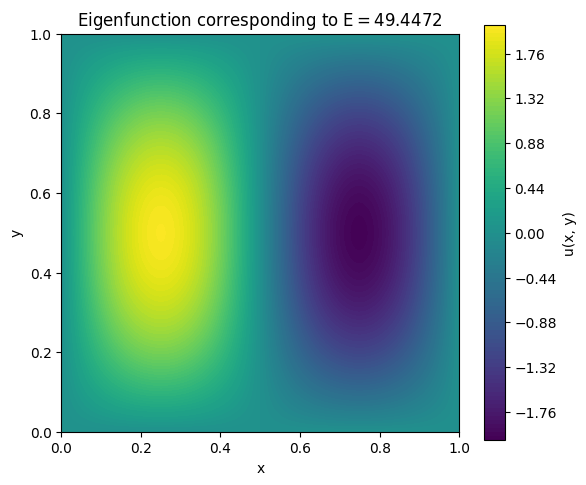
\includegraphics[width=.24\textwidth]{n=2_p=2_v=0_mu=150_cuadrado_autof2.png}
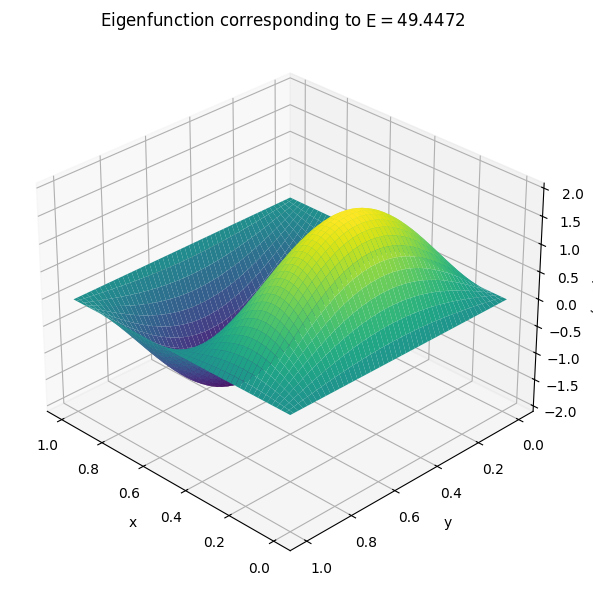
\includegraphics[width=.24\textwidth]{n=2_p=2_v=0_mu=150_cuadrado_autof23d.png}
\caption{The first two computed eigenfunctions in the unit square (from a run with $\mu=150$).}
\label{loss.lap.square.fig.2}
\end{minipage}
\end{figure}

\subsection{Triangle and annulus}
The Dirichlet eigenfunctions of the triangle with vertices $(0,0)$, $(1,0)$, $(0,1)$ are
$\sin(m\pi x_1)\sin(n\pi x_2)-(-1)^{m+n}\sin(n\pi x_1)\sin(m\pi x_2)$, $m>n\ge1$, with eigenvalue
$\pi^2(m^2+n^2)$; all the eigenvalues in the window $[0,180]$ are simple. The full scan uses
$\mu=15000$ (Figs.~\ref{loss.lap.triang.fig} and \ref{loss.lap.triang.fig.2}). Table~\ref{table.4}
compares the exact eigenvalues with values computed on three-node windows as for the balls. Here the
first (cold) node of every window failed to converge within 2000 epochs at $\mu=15000$ ($\hat E=56.0$,
$57.1$, $88.0$, $164.7$ with $r=15$--$62$, i.e.\ a wrong branch), and the values come from the second or
third node; the residuals are larger than in the full warm-started scan of
Fig.~\ref{loss.lap.triang.fig}, but all rows satisfy the Weinstein bound. In the annulus
$\{0.5<|x|<1\}$ (Fig.~\ref{loss.lap.annulus.fig}) the scan followed the radial branch and missed two
eigenvalues, an instance of a branch-switched (lagging) scan (Appendix~\ref{sec.analysis}).

\begin{table}[H]
\centering\small
\caption{Eigenvalues of problem \eqref{eigen2} in the triangle with vertices $(0,0)$, $(1,0)$, $(0,1)$ compared with the exact values (three-node windows, $\mu=15000$, seed 0). All the eigenvalues listed are simple; these are all the eigenvalues in $[0,180]$. $\hat E$ with Monte Carlo standard error; $r$: Weinstein radius.}
\label{table.4}
\begin{tabular}{ccccc}
\toprule
$(m,n)$ & $E_{(m,n)} = \pi^2 (m^2 + n^2)$ & $\hat E$ & rel.\ error & $r$\\
\midrule
$(2,1)$ & $5\pi^2\approx 49.3480$ & 49.3509(14) & $5.8\times10^{-5}$ & 0.94\\
$(3,1)$ & $10\pi^2\approx 98.6960$ & 98.7067(24) & $1.1\times10^{-4}$ & 1.81\\
$(3,2)$ & $13\pi^2\approx 128.3049$ & 128.4612(95) & $1.2\times10^{-3}$ & 5.68\\
$(4,1)$ & $17\pi^2\approx 167.7833$ & 167.7923(35) & $5.4\times10^{-5}$ & 2.51\\
\bottomrule
\end{tabular}
\end{table}

\begin{figure}[H]
\centering
\begin{minipage}[t]{.4\textwidth}
\centering
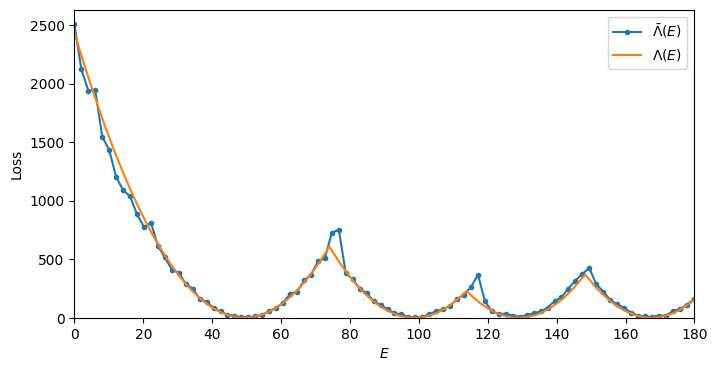
\includegraphics[width=\textwidth]{loss_n=2_p=2_V=0_mu=15000_triangulo.png}
\caption{The loss curve $\bar\Lambda(E)$ in the triangle with vertices $(0,0)$, $(0,1)$, $(1,0)$ compared with the exact curve.}
\label{loss.lap.triang.fig}
\end{minipage}\hfill
\begin{minipage}[t]{.56\textwidth}
\centering
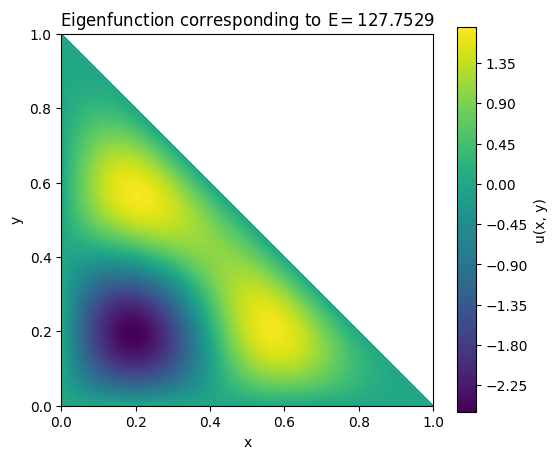
\includegraphics[width=.24\textwidth]{eigen_p=2_n=2_V=0_triangulo_4.png}
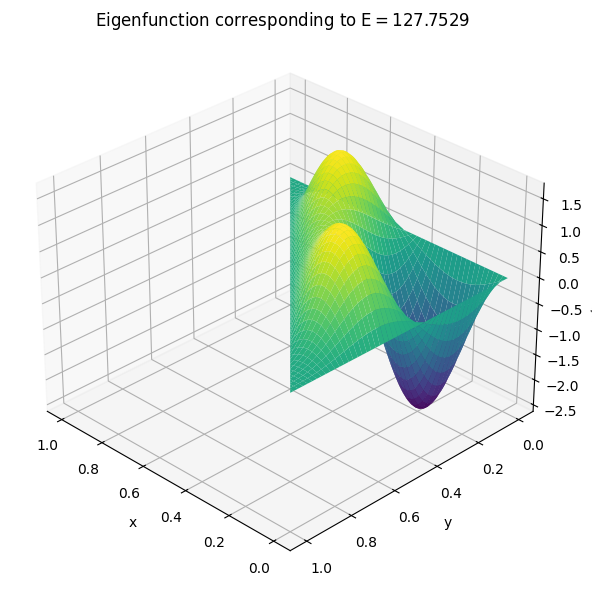
\includegraphics[width=.24\textwidth]{eigen_p=2_n=2_V=0_triangulo_4_3d.png}
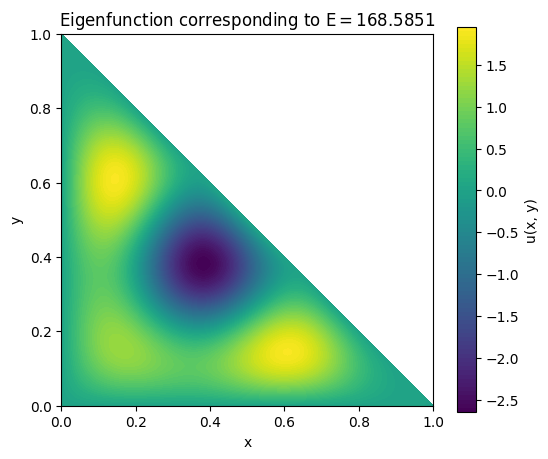
\includegraphics[width=.24\textwidth]{eigen_p=2_n=2_V=0_triangulo_5.png}
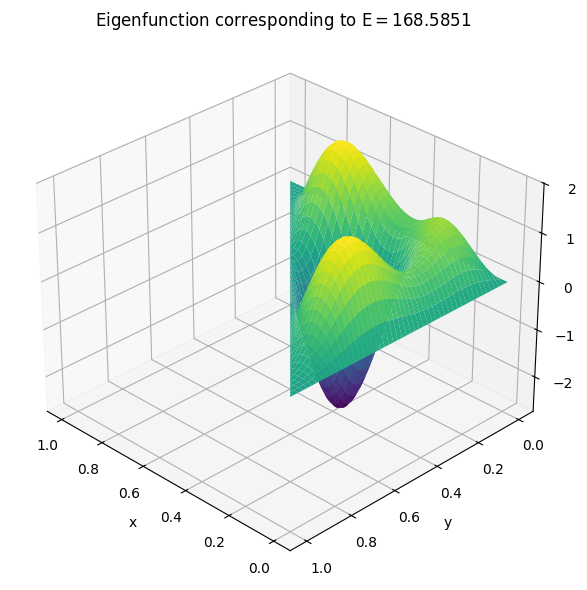
\includegraphics[width=.24\textwidth]{eigen_p=2_n=2_V=0_triangulo_5_3d.png}
\caption{Third and fourth computed eigenfunctions in the triangle with vertices $(0,0)$, $(0,1)$, $(1,0)$ (from a different run than Table~\ref{table.4}; the panel titles show the values of that run).}
\label{loss.lap.triang.fig.2}
\end{minipage}
\end{figure}

\begin{figure}[H]
\centering
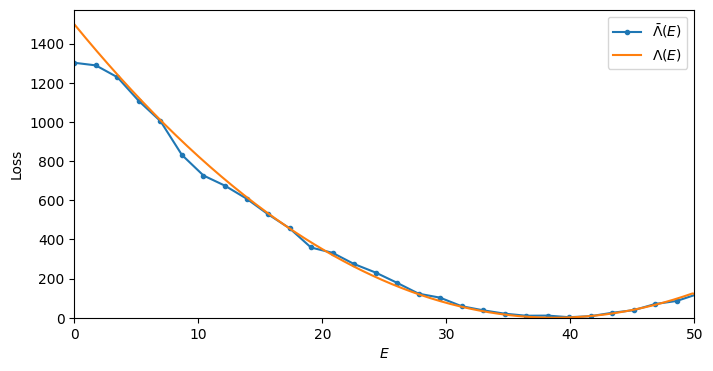
\includegraphics[width=.26\columnwidth]{loss_n=2_p=2_V=0_annulus.png}
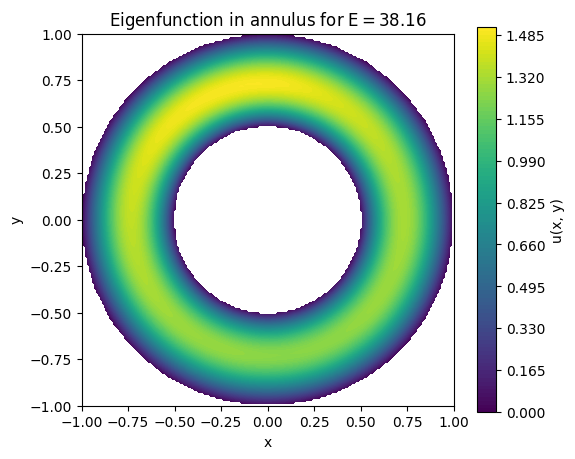
\includegraphics[width=.26\columnwidth]{eigen1-annulus.png}
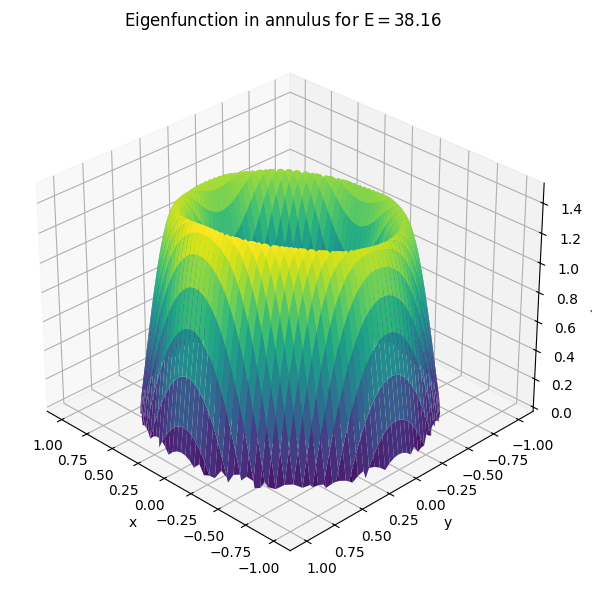
\includegraphics[width=.26\columnwidth]{eigen1-3d-annulus.png}
\caption{Left: the loss curve $\bar\Lambda(E)$ in the annulus $\{0.5<|x|<1\}$; the reference curve drawn in this plot contains only the first eigenvalue $39.0133$, whereas the window also contains $40.8725$ (double) and $46.4285$ (double). The PINN scan followed the radial branch and missed these two eigenvalues (an example of a missed eigenvalue, see Appendix~\ref{sec.analysis}). Centre and right: the first computed eigenfunction.}
\label{loss.lap.annulus.fig}
\end{figure}

\subsection{Potentials}\label{sec.potentials}
The problem is always solved in the unit disk or ball with Dirichlet boundary condition. We consider
the harmonic potential $V(x)=\frac{\omega^2}{2}|x|^2$ in the unit disk for $\omega=1$
(Fig.~\ref{pot2.fig}) and $\omega=10$ (Fig.~\ref{pot1.fig}); because of the boundary condition, this is
not the harmonic oscillator on $\R^2$. The double-well Gaussian potential in the unit ball of $\R^3$ is
\[
V(x)=-V_0\Big(e^{-|x-ae_1|^2/(2\sigma^2)}+e^{-|x+ae_1|^2/(2\sigma^2)}\Big),\qquad a=1,\ \sigma=0.5,\ V_0=1,
\]
i.e.\ $V(x)=-e^{-2|x-x_0|^2}-e^{-2|x+x_0|^2}$ with $x_0=e_1=(1,0,0)$; the centres of the wells lie on the
boundary sphere. For the four-well compactly supported potential in the unit ball of $\R^3$, let the
centres of the wells be $z_1 = (a,a,0)$, $z_2 = (-a,a,0)$, $z_3 = (a,-a,0)$, $z_4 = (-a,-a,0)$, where
$a=0.22$, let $\sigma=0.2$, and define $\phi(t) =\exp(-(1-t^2)^{-1})$ for $t < 1$ and $\phi(t)=0$ for $t \ge 1$.
Then
$
V(x) = - \sum_{i=1}^{4} \phi\big( |x - z_i|/\sigma \big)
$
(depth $e^{-1}\approx0.37$ at each centre). The loss curves of both well potentials are shown in
Fig.~\ref{fig.well-two}. In the harmonic, double-well and four-well examples we used $\mu=100$, $400$ and
$1000$, respectively (2000 sampling points for the four-well potential).

\begin{figure}[H]
\centering
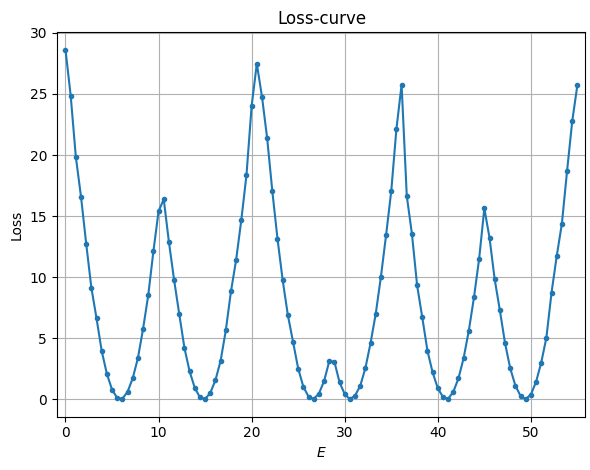
\includegraphics[width=.26\columnwidth]{loss_p=2_n=2_V=harmonic_omega=1_disco.png}
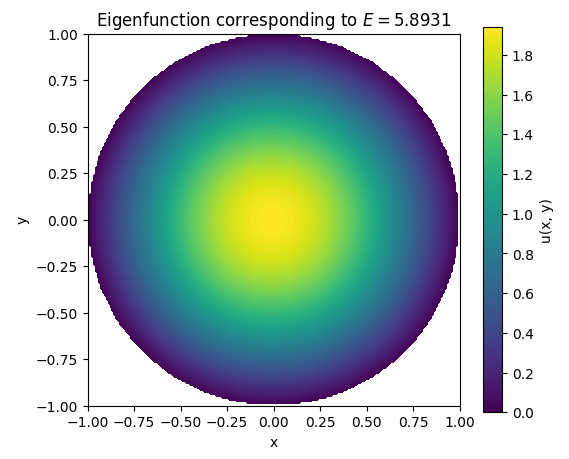
\includegraphics[width=.26\columnwidth]{egen_p=2_n=2_V=harmonic_omega=1_disco_1.png}
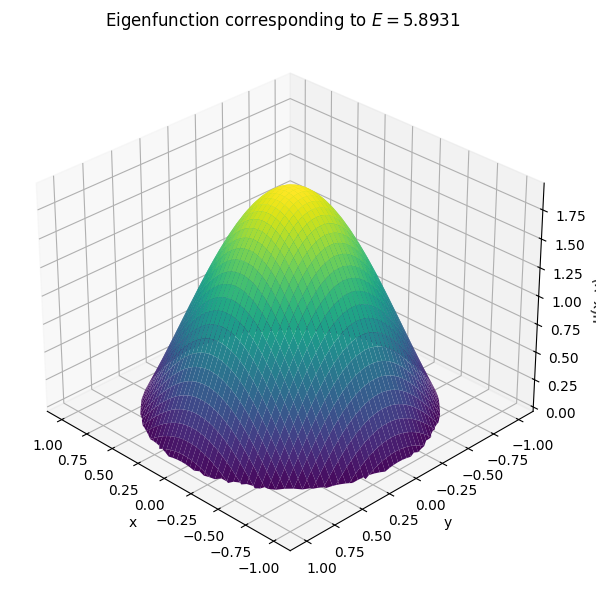
\includegraphics[width=.26\columnwidth]{egen_p=2_n=2_V=harmonic_omega=1_disco_1_3d.png}
\caption{The loss curve $\bar\Lambda(E)$ in the unit disk with harmonic potential $V=\frac{\omega^2}{2}|x|^2$ and $\omega=1$ with the first computed eigenfunction. The finite element eigenvalues in the window (Appendix~\ref{app.fem}) are $5.8919$, $14.8484$ (double), $26.5790$ (double), $30.6271$, $40.9385$ (double), $49.3852$ (double); the minima of this curve were not refined.}
\label{pot2.fig}
\end{figure}

\begin{figure}[H]
\centering
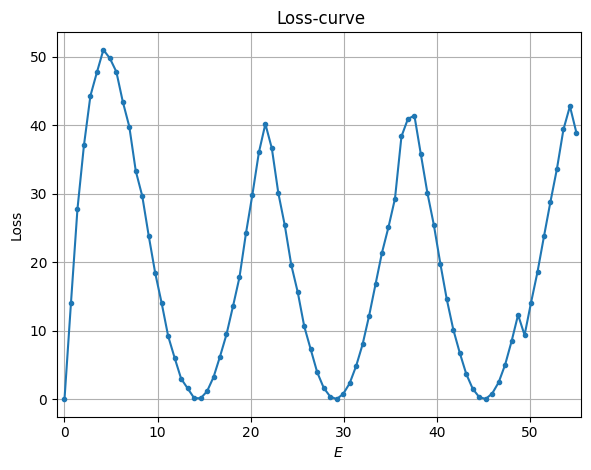
\includegraphics[width=.26\columnwidth]{loss_n=2_V=harmonic_p=2.png}
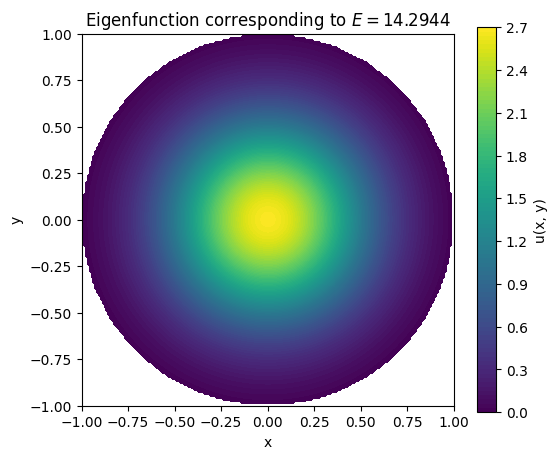
\includegraphics[width=.26\columnwidth]{eigen_n=2_V=harmonic_p=2_1.png}
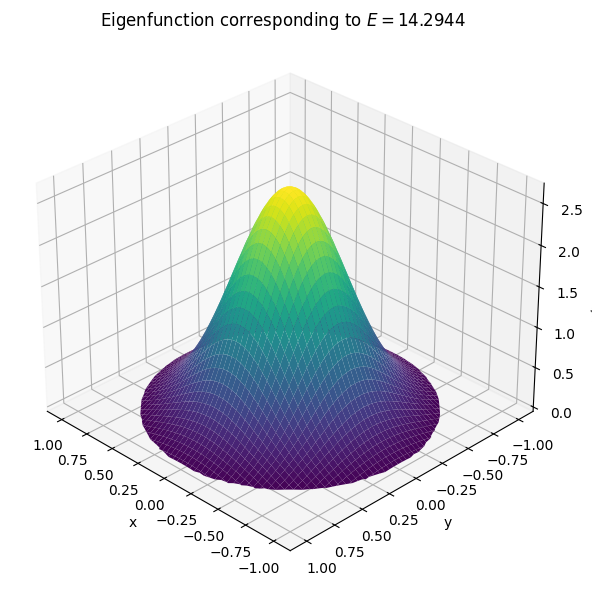
\includegraphics[width=.26\columnwidth]{eigen_n=2_V=harmonic_p=2_1_3d.png}
\caption{The loss curve $\bar\Lambda(E)$ in the unit disk with harmonic potential $V=\frac{\omega^2}{2}|x|^2$ and $\omega=10$ with the first computed eigenfunction. The eigenvalues in the window are $14.2847$, $29.1349$ (double), $45.0887$ (double), $46.2907$; the last two are $1.2$ apart and appear as a single minimum in this scan (grid step $\approx0.7$; with step $0.5$ they are separated, Appendix~\ref{app.fem}). The value $\bar\Lambda=0$ at $E=0$ is the trivial state $u=0$ ($\ell(0)^2=204>2\mu=200$, Proposition~\ref{prop.penalized}).}
\label{pot1.fig}
\end{figure}

\begin{figure}[H]
\centering
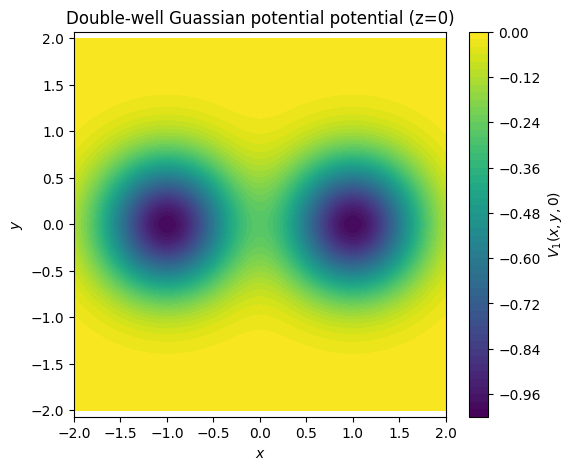
\includegraphics[width=.24\columnwidth]{well-1.png}
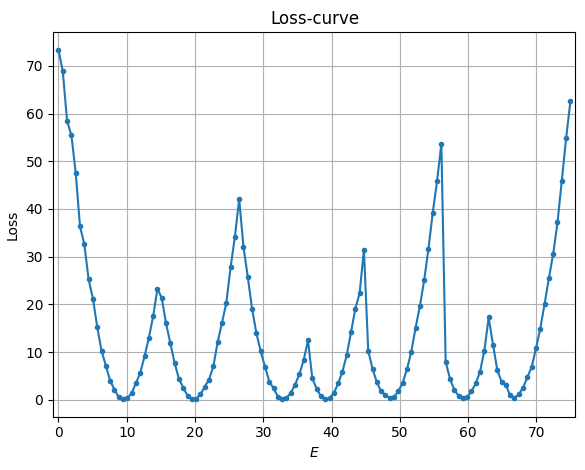
\includegraphics[width=.24\columnwidth]{well-1-plot.png}
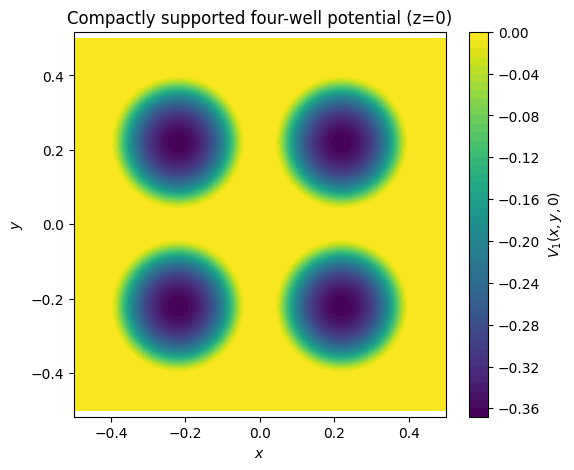
\includegraphics[width=.24\columnwidth]{well-2.png}
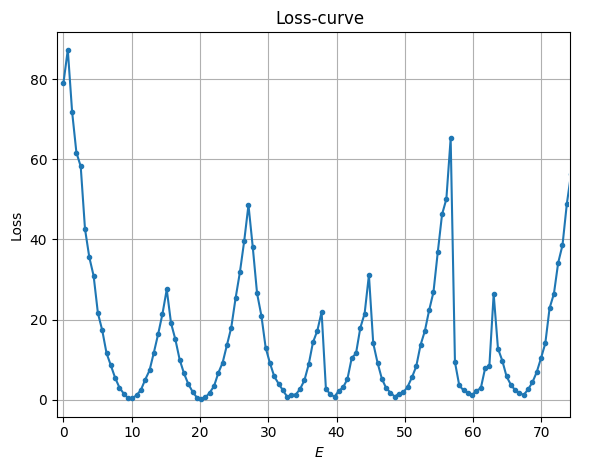
\includegraphics[width=.24\columnwidth]{well-2-plot.png}
\caption{Unit ball of $\R^3$. Left half: double-well Gaussian potential and loss curve $\bar\Lambda(E)$; right half: compactly supported four-well potential and loss curve.}
\label{fig.well-two}\label{fig.well-four}
\end{figure}

\subsection{Finite element validation}\label{app.fem}
\emph{Reference method.} Lagrange $P_2$ elements on curved (isoparametric) meshes, generalized
eigenvalue problem solved by shift-invert Lanczos, Richardson extrapolation over the last three uniform
refinements. The finite element code reproduces the exact eigenvalues of the disk, annulus, square and
triangle with errors $10^{-10}$--$10^{-6}$ (observed order $4$ in two dimensions) and those of the ball of
$\R^3$ with errors $7\times10^{-5}$ to $1.6\times10^{-2}$ for $E\le67$ (observed order $\approx2.8$, three
mesh levels with up to $41\,727$ degrees of freedom); the reported uncertainty of the extrapolated values
is conservative on these test cases.

\emph{Centred windows.} For each potential we trained the PINN on four windows of seven grid points (step
$0.5$), with the settings of Table~\ref{table.settings} and 2--3 seeds; the eigenvalue is the Rayleigh
quotient of the network at the node of smallest normalized loss. \emph{The windows were centred at the
finite element values}: this is a test of the accuracy of the loss curve at known eigenvalues, not a
blind detection (the blind scan is Table~\ref{table.blind}). Table~\ref{table.fem} and Fig.~\ref{fig.fem}
show the results (Table~\ref{table.fem} is in Section~\ref{sec.fem}). Since the reference values are themselves approximations, we speak of relative
differences.


\begin{figure}[H]
\centering
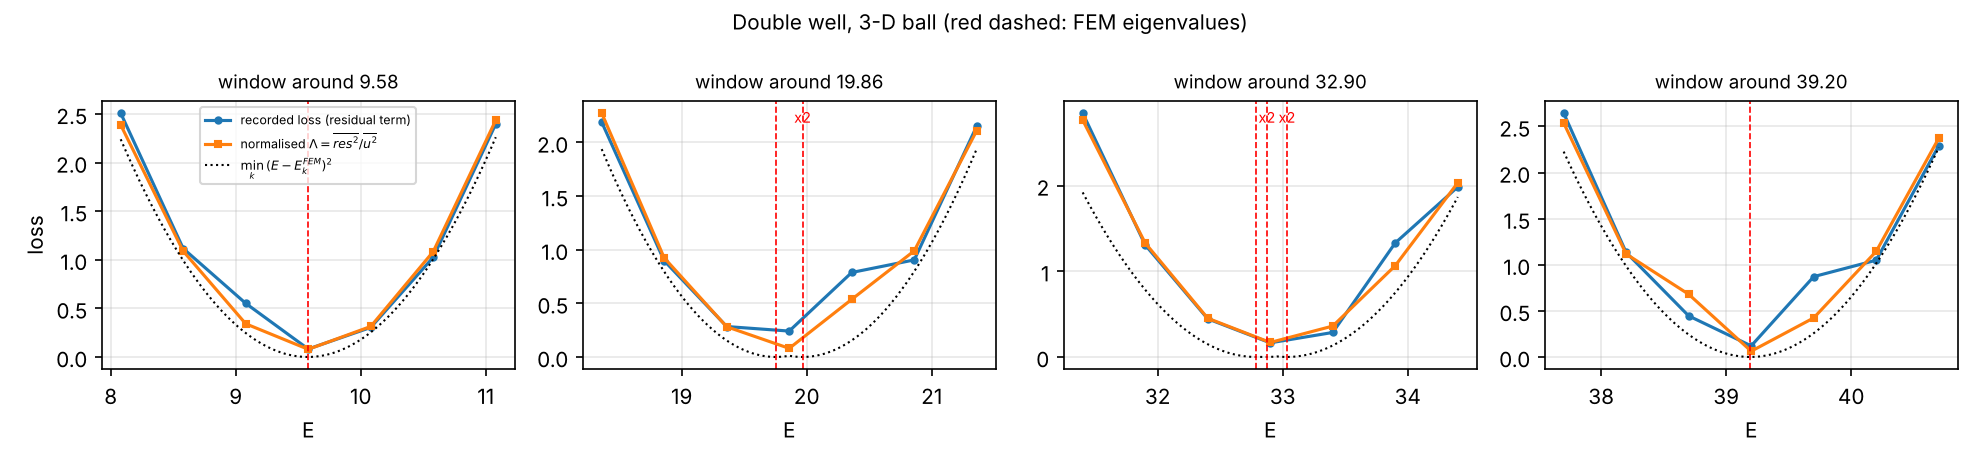
\includegraphics[width=.62\textwidth]{pinn_vs_fem_double_well.png}\\
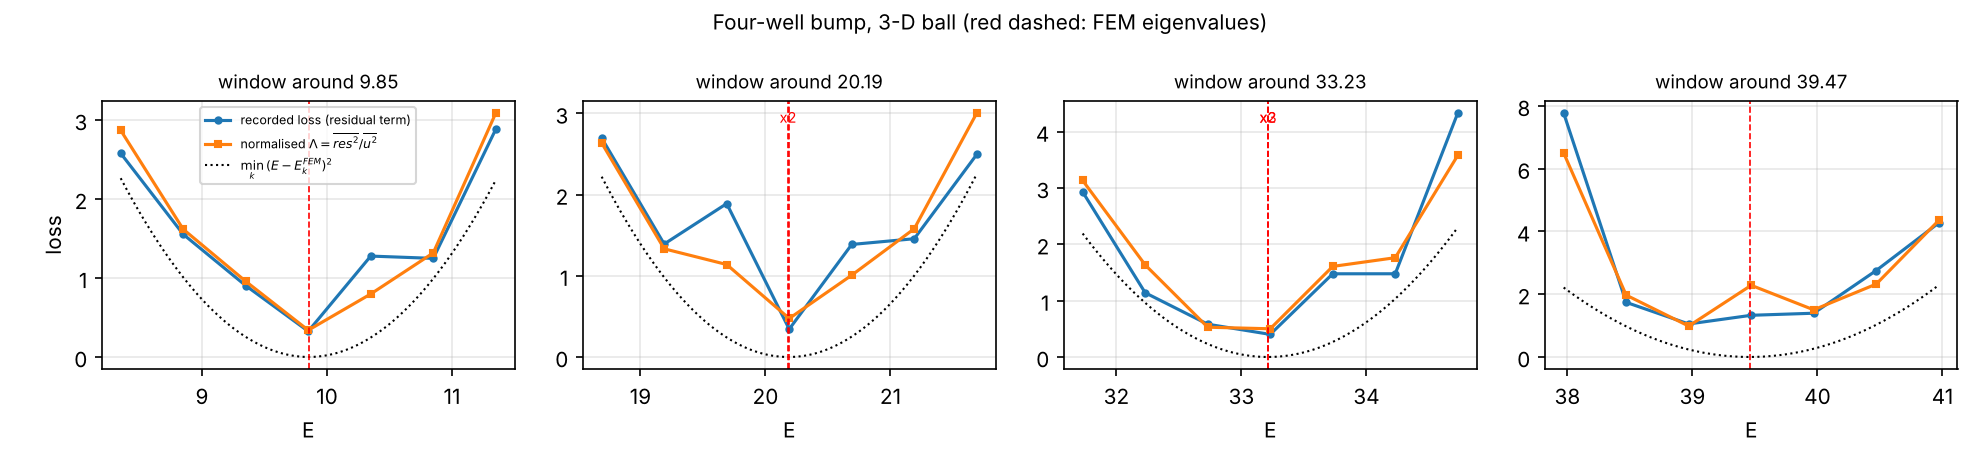
\includegraphics[width=.62\textwidth]{pinn_vs_fem_four_well.png}\\
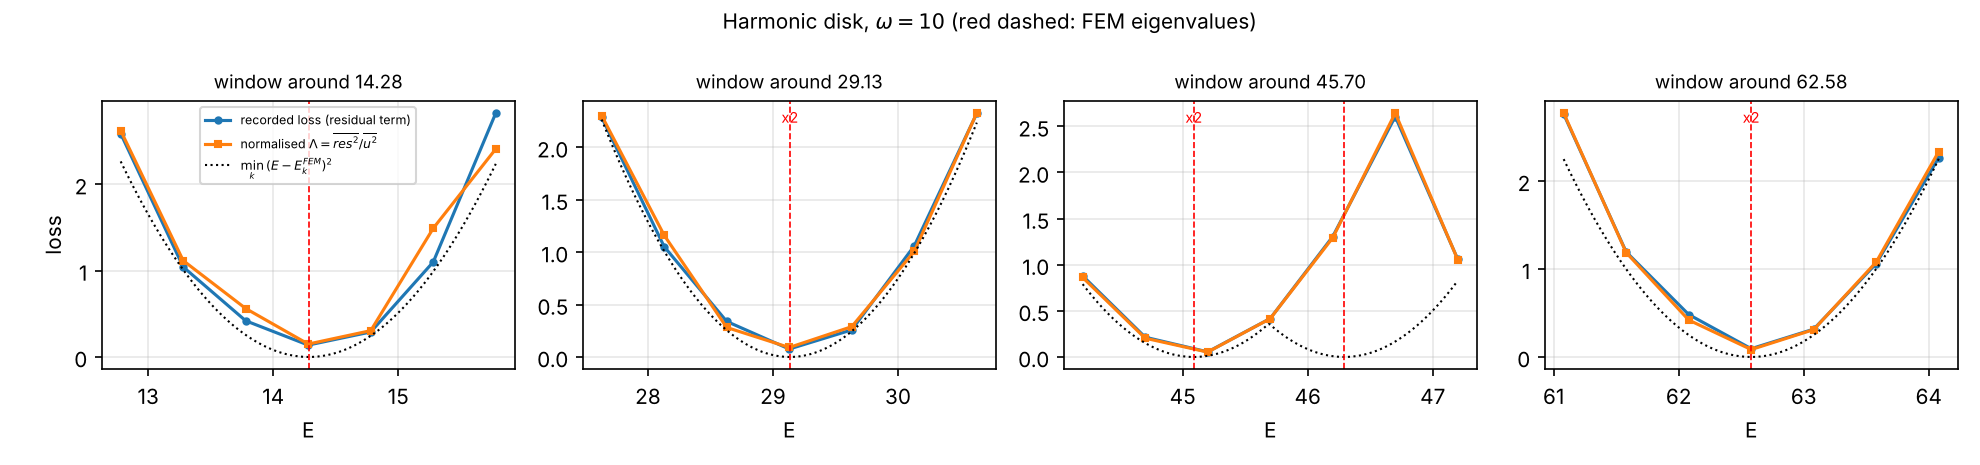
\includegraphics[width=.62\textwidth]{pinn_vs_fem_harm_w10.png}
\caption{PINN loss curves on windows centred at finite element eigenvalues (red dashed lines; ``x2'': double) for the double-well (top), four-well (middle) and harmonic $\omega=10$ (bottom) potentials: recorded residual term, normalized loss $\Lambda$, and $\min_k(E-E_k^{\rm FEM})^2$ (dotted).}
\label{fig.fem}
\end{figure}

\emph{Findings.} (i) The seed means agree with the finite element values to within $0.1\%$ and single
runs to within $0.25\%$; the largest single-run difference ($+0.25\%$, double well near $32.9$) occurs in
a window containing three eigenvalues spread over $0.25$, and lies inside the cluster; outside clusters
the largest difference is $0.105\%$ (four well, $9.85$). In three dimensions the finite element
uncertainty ($5\times10^{-4}$ to $2\times10^{-2}$) is comparable to the differences, and in three of the
eight windows it exceeds them. The minimum of the loss is not zero ($\min\Lambda=0.06$--$1.05$, i.e.\
$r=0.25$--$1$): as explained in Section~\ref{sec.certificate}, the accuracy comes from the Rayleigh
quotient, whose error is quadratic in $r$. (ii) The spectra of the well potentials consist of
\emph{clusters of close eigenvalues}: for the double well $19.75$ and $19.97$ (double), and $32.79$,
$32.87$ (double), $33.03$ (double); for the four well $20.180$ (double) and $20.189$, and $33.210$
(double) and $33.214$ (triple). The loss curve has one minimum per cluster and the quotient returns a
value inside the cluster; the number of eigenvalues in the cluster and their multiplicities cannot be
read from the curve (see Remark~\ref{rem.stability}). The blind scan of Table~\ref{table.blind} confirms
this. (iii) The well potentials are weak perturbations of the free ball: the first eigenvalue moves from
$\pi^2=9.8696$ to $9.5764$ (double well) and to $9.8542$ (four well); for the four-well potential the
shift is of the same order as the PINN differences, so this example hardly distinguishes the potential
from $V=0$. (iv) In the harmonic case with $\omega=10$, the double eigenvalue $45.0887$ and the simple
eigenvalue $46.2907$ are $1.2$ apart. With warm start the network stays on the branch of $45.09$ up to
$E\approx46.2$--$46.7$ and then switches to $46.29$ (quotient $46.289$--$46.291$ at the last nodes of both
seeds). On a window extended to $49.2$ (step $0.5$, seed 0) the normalized loss has two separate minima,
at $E=45.2$ ($\hat E=45.093$) and at $E=46.2$ ($\hat E=46.2903$), separated by a ridge at $45.7$; with the
coarser step $\approx0.7$ of Fig.~\ref{pot1.fig} this hysteresis hides the second eigenvalue. (v) For
these linear problems the finite element method is much cheaper and more accurate (timings in
Section~\ref{sec.fem}); the purpose of the method is not to compete with finite elements on linear
problems in low dimension.

% ---------------------------------------------------------------------------
\section{The penalty parameter \texorpdfstring{$\mu$}{mu}}\label{sec.mu}

Corollary~\ref{cor.mu} concerns the recorded residual $\mathcal R_\mu$, which is the quantity that is
thresholded; the location of the minima of $\bar\Lambda$ and the normalized quotient
$\Lambda(u_E,E)=\ell(E)^2$ do not depend on $\mu$. The settings of all our examples are compared with the
rule $\mu\ge D^2$ in Table~\ref{table.settings}: it holds in all of them except the ball of $\R^4$ (regime
(iii), $\mu=200<D^2=216$) and the harmonic potential with $\omega=10$ (regime (iv), collapse at $E=0$,
Fig.~\ref{pot1.fig}); in the triangle, for instance, the window $[0,180]$ starts far below $E_1=5\pi^2$, so
$D=5\pi^2$ and $D^2\approx2435<\mu=15000$. Training from scratch at a high level $E$ (cold start, or
periodic re-initialization) is discussed in Appendix~\ref{app.cold}.

\emph{Test of the rule.} We used a reduced network ($3\times64$, 3000 points, at most 2000 epochs; at
$\mu=1000$ it gave the same normalized loss values and Rayleigh quotients as the full network to within
the training noise), warm start and two seeds. On the window $[15,55]$ of the unit square, which
contains $2\pi^2$ and $5\pi^2$ (double), $D=14.8$ at the mid-gap $34.5$ and $D^2=219.2$, we used an offset
grid $E=15.6,18.1,\dots,53.1$ (no node on an eigenvalue) and six values of $\mu$ (Table~\ref{table.mu}, Section~\ref{sec.approach}).
The predicted effect is observed: for $\mu<D^2$ the recorded residual has a spurious interior minimum in
the gap ($E\approx33$--$36$, next to the mid-gap) in all six runs, and for $\mu\ge D^2$ in none of the six
runs; for $\mu<D^2/2$ the network collapses exactly at the predicted nodes. The eigenvalues themselves
are located correctly for every $\mu$ (Rayleigh quotient within $2\times10^{-3}$ of $2\pi^2$ and $10^{-3}$ of
$5\pi^2$), and the normalized loss $r^2$ has no spurious minimum for $\mu\ge75$: the rule concerns the
recorded residual that is thresholded, not the eigenvalue estimate. On the window $[40,60]$, which
contains only $5\pi^2$ ($D^2=113.5$, step 2, nine values of $\mu$ from $1$ to $10^4$), the recorded curves
follow the closed form of Proposition~\ref{prop.penalized} for $60\le\mu\le1000$ (Fig.~\ref{fig.mu}; the
mean of $u^2$ follows $1-\ell^2/(2\mu)$ with an RMS deviation $\approx0.01$ for $\mu\ge100$); the networks
collapse at the far nodes for $\mu<D^2/2$ (at all nodes for $\mu=1,10$, more than predicted, because a
warm-started $u\approx0$ is not left, and at $\mu=30$ the collapsed state carried along by the warm start
produces a spurious zero at $E=42$); the relative error of the eigenvalue is at most $2.9\times10^{-5}$ for
$60\le\mu\le1000$ and $2.0\times10^{-4}$ for $\mu=10^4$, where the curve is distorted (stiff penalty). A
single eigenvalue gives a single basin, so this window cannot distinguish $\mu=60$ from $\mu=113$.


\begin{figure}[H]
\centering
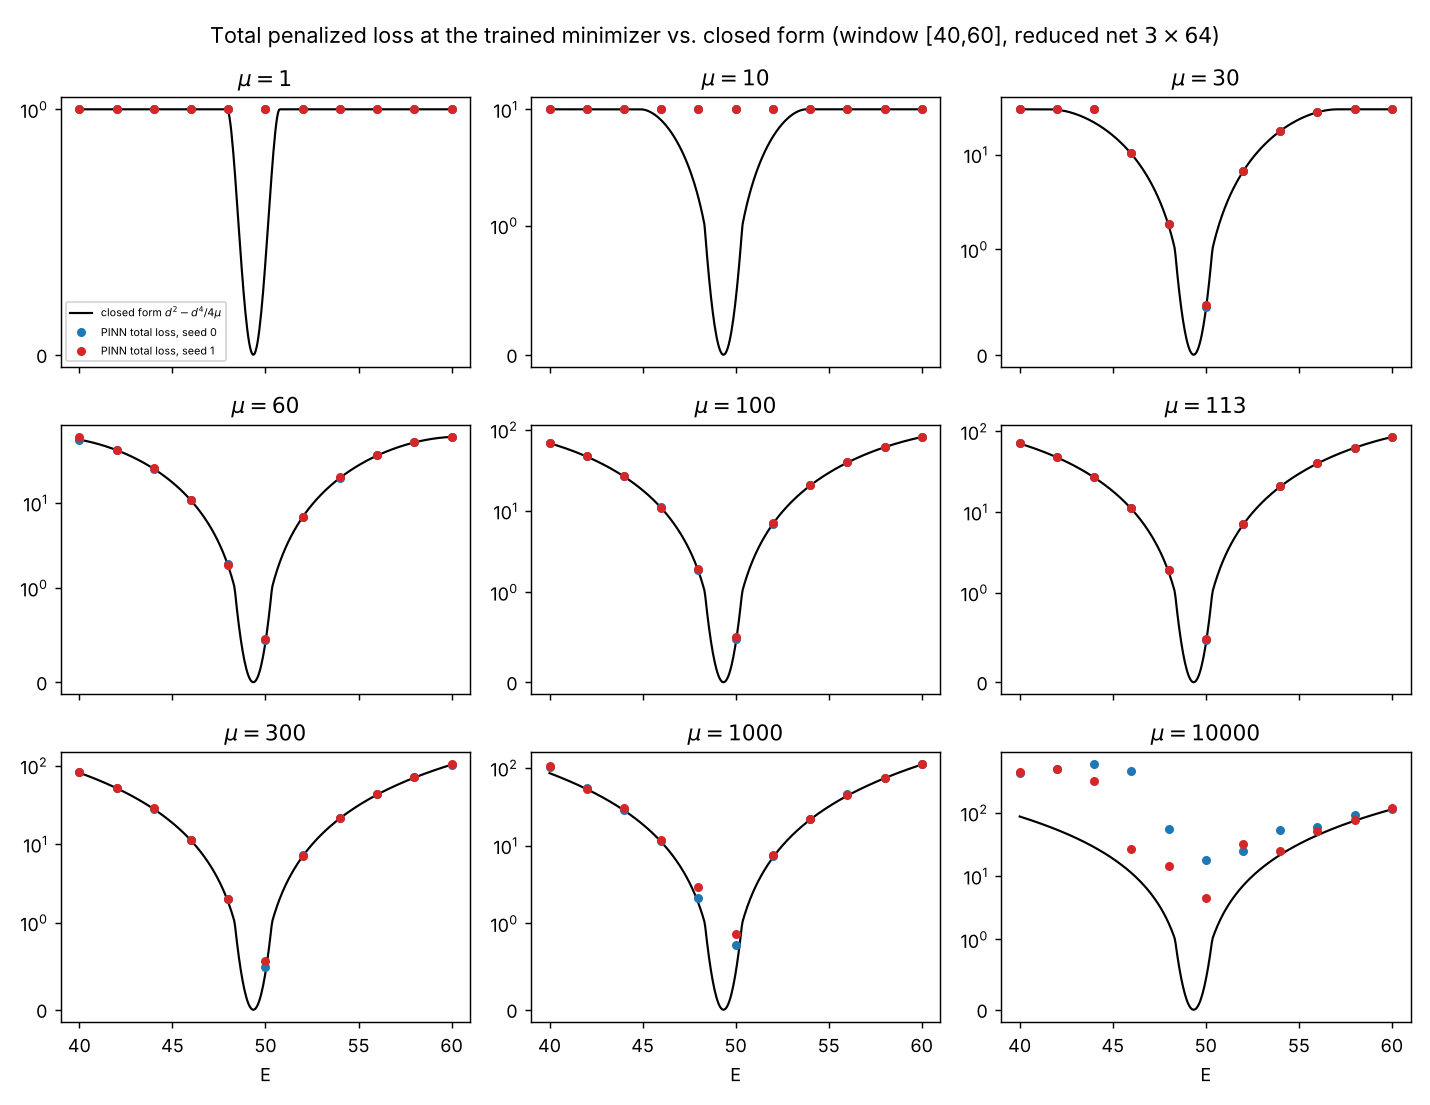
\includegraphics[width=.45\textwidth]{mu_loss_curves.png}
\caption{Total penalized loss at the trained networks (dots, two seeds) and the closed form $\ell^2-\ell^4/(4\mu)$ of Proposition~\ref{prop.penalized} (solid line), window $[40,60]$ of the unit square, for nine values of $\mu$ between $1$ and $10^4$.}
\label{fig.mu}
\end{figure}

% ---------------------------------------------------------------------------
\section{Stability measurements, cold start and refinement}\label{sec.analysis}
This appendix reports the measurements behind Section~\ref{sec.stability}, the behaviour of cold starts, and the comparison of refinement estimators.

\subsection{Error decomposition and interpretation}\label{app.stab}
The error of the computed loss at the node $E^i$ splits as
\[
\tilde\Lambda_i-\Lambda(E^i)=
\underbrace{\Lambda(u^i,E^i)-\inf_{\mathcal N}\Lambda(\cdot,E^i)}_{\text{optimization}\ \ge0}
+\underbrace{\inf_{\mathcal N}\Lambda(\cdot,E^i)-\Lambda(E^i)}_{\text{approximation}\ \ge0}
+\underbrace{\tilde\Lambda_i-\Lambda(u^i,E^i)}_{\text{sampling}} ;
\]
hypothesis \eqref{hyp.delta} bounds the total. Since $\tau\ge\sqrt{2\delta}$, part (d) of
Proposition~\ref{prop.stability} can only apply to eigenvalues whose distance $\gamma$ to the rest of the
spectrum satisfies roughly $\delta\ll\gamma^2/8$; the proposition is informative only in this regime,
which we check below.

\begin{remark}[Interpretation]\label{rem.stability}
(1) Imperfect training cannot create detections far from the spectrum: every node below the
threshold, and every discrete local minimum, lies within an explicit distance of a true
eigenvalue, provided \eqref{hyp.delta} holds. What it can do is produce several minima around the
same eigenvalue, or raise the curve above the threshold so that an eigenvalue is missed. Refining the
grid below $h\simeq\sqrt{2\delta}$ does not improve the localization (the bound in (c) is minimal
there). (2) The loss curve only sees the set $\sigma$: a multiple eigenvalue produces a single
minimum and the network converges to some element of the eigenspace. Multiplicities would have to
be recovered separately, e.g.\ by training at the detected value from several initializations and
computing the rank of the Gram matrix of the resulting functions; we have not implemented this.
(3) Two eigenvalues are separated by a bump of height $(E_{k+1}-E_k)^2/4$; if
$E_{k+1}-E_k\le2\sqrt{2\delta}$ the bump is below the error level and the number of eigenvalues in
such a cluster cannot be determined from the curve: the method returns the cluster as a single
approximate eigenvalue (Section~\ref{sec.fem}). (4) Proposition \ref{prop.stability} is conditional
on \eqref{hyp.delta}; we do not prove a bound on $\delta$ in terms of the network size, the number of
epochs and of sampling points. The approximation error tends to zero as the width grows (networks
with smooth non-polynomial activation are dense in $C^2(\overline\Omega)$
\cite{Hornik1991,Pinkus1999}; rates for $\tanh$ networks are given in
\cite{DeRyck-Lanthaler-Mishra}), but no convergence guarantee for the optimizer is available, and the
spectral bias of gradient-based training \cite{Rahaman-etal} suggests that $\delta$ grows with $E$,
in agreement with the residuals in our tables. The error can, however, be \emph{measured} a
posteriori, as we do next.
\end{remark}

\subsection{Experiments}
(i) \emph{Seeds and certificates.} The three seeds on the window $[15,55]$ of the unit square and the
ratios between the certificates and the actual errors over the 14 minima detected in our unit-square
runs (these scans, the scan of Table~\ref{table.1} and the cold-start runs) are reported in
Section~\ref{sec.examples}.

(ii) \emph{Size of $\delta$.} We measured $\delta_i=|r_i^2-\ell(E^i)^2|$ at every node, with $r_i^2$ the
normalized loss on a fresh sample. In the three seeds of the offset scan of Table~\ref{table.cost}
(18 nodes on $[17.3,102.3]$) the maxima were $3.5$, $2.9$, $2.6$; in the three seeds on $[15,55]$ they
were $9.8$, $7.8$, $12.1$, attained at the mid-gap node $E=35$, where $\ell^2\approx206$ and a relative
error of a few percent in $r^2$ gives $\delta\approx10$ (medians $0.15$--$0.25$). In the 80-node scan of
Table~\ref{table.1} the maximum over all nodes was $1749$, but after excluding $9$ nodes (5 collapsed,
4 branch-switched or lagging nodes: after the re-initialization at $E\approx66.5$ the network sat on the
$5\pi^2$ branch, and already at $E=65.1$, past the mid-gap $64.15$, the warm-started network had
lagged on that branch) it was $2.35$ (median $0.26$). On the remaining (clean) nodes $\delta\le12.1$, well
below $\gamma^2/8=48.7$ and $109.6$ for the gaps $\gamma=19.7$ and $29.6$ of the unit square, and the
hypotheses of (d) hold (e.g.\ $h=5$, $\delta=12.1$ give $2\tau+h=16.0<19.7$). They do not make the bound
(c) sharp: $\delta$ is comparable to $h^2/4$ at the mid-gap nodes, where it is dominated by the training
floor at large $\ell$. Large values of $\delta$ occurred only at collapsed nodes and at branch-switched or
lagging nodes, where the network sits on the eigenfunction of an eigenvalue different from the nearest
one; the eigenvalues missed in the annulus and for $\omega=10$ (Appendix~\ref{app.fem}) are instances of
the second kind. Both are visible in the network itself: the first by a vanishing mass, the second by a
jump of the Rayleigh quotient along the scan.

(iii) \emph{Collapse.} Spurious zeros of the \emph{recorded} curve were observed, but only in one form:
the collapse to the trivial state $u\equiv0$. In the scan of Table~\ref{table.1} the network was
re-initialized at $E=99.7$, collapsed to $u\equiv0$ and stayed there up to $E=105$
(Fig.~\ref{fig.collapse}). The recorded residual term dropped to $\approx10^{-5}$, the lowest value of
the whole curve, which any threshold would accept; but the mean of $u^2$ was $\approx10^{-8}$ and the
certificate radius $r$ was $30$--$42$. Collapsed nodes are therefore detected by $\overline{u^2}\approx0$
and a large $r$, and are invisible in the residual term alone. The same happens when $\mu$ is too small
(Appendix~\ref{sec.mu}). We therefore record, at each node, the normalized loss $\Lambda(u,E)=r^2$, the
mass $\overline{u^2}$ and the Rayleigh quotient, and discard nodes with $\overline{u^2}<\frac12$.


\subsection{Cold start}\label{app.cold}
When the network is trained from scratch at a level $E$, the residual of the initial network is of order
$E^2$ and the amplitude is driven towards $u=0$ unless, heuristically, $\mu\gtrsim\frac12E^2$. On the
window $[95,102]$ (five nodes, fresh network at the first node, then warm start, at most 5000 epochs)
the eigenvalue $10\pi^2$ was reached as follows: $\mu=450$: collapse at all nodes (one seed); $\mu=3000$:
only at the last node, the first four nodes converged to the eigenfunction of $5\pi^2$ (one seed; similar
failures at $8\pi^2$ and $10\pi^2$ in two further cold chains); $\mu=5000\approx E^2/2$: at 8 of 15 nodes
(three seeds; the other nodes on the $5\pi^2$ branch); $\mu=20000$: at none of 15 nodes (all stuck at
$2\pi^2$). Thus $\mu\gtrsim E^2/2$ avoids collapse but is not sufficient, and cold start at a high level is
unreliable: the network tends to fall into the eigenfunction of a lower eigenvalue and only sometimes
leaves it. The re-initializations of the scan of Table~\ref{table.1} ($\mu=500\ll E^2/2$) show the same:
branch switch at $E\approx66$ and collapse at $E\ge99.7$. In the local windows of
Tables~\ref{table.2}--\ref{table.4} the cold first node converged in the ball of $\R^3$ but failed in every
window of the triangle. We therefore recommend warm-start continuation from a window that starts at or
below the target, or several independent restarts, and accepting a detection only through the mass,
the Rayleigh quotient and the certificate.

\subsection{Refinement estimators and Monte Carlo errors}\label{app.refine}
The minimizer of $E\mapsto\Lambda(u^{i_0},E)$ could also be computed by a bounded scalar minimization of
the Monte Carlo objective re-sampled at every evaluation, but a stochastic objective of this kind is
flat to within its noise, and the returned value has an error of order the square root of the noise
level. Evaluating the closed form $\rho(u^{i_0})$ on a fixed sample is both cheaper and more accurate: on
14 minima detected in the unit square the median absolute error was $6.6\times10^{-3}$ with the
re-sampled minimization, $1.1\times10^{-3}$ with the closed form on $10^5$ fixed Monte Carlo points and
$6.6\times10^{-4}$ on a $300\times300$ midpoint grid (maximal errors $1.3\times10^{-1}$, $5.5\times10^{-3}$,
$5.8\times10^{-3}$); a three-point parabolic fit of the loss values at coarse nodes was not reliable
(median $9.7\times10^{-3}$, maximum $1.0$), because different nodes carry different training floors. We use
the form $-\int u(\Delta u-Vu)/\int u^2$: on $4\times10^5$ Monte Carlo points its standard error was
$2\times10^{-4}$--$2.4\times10^{-3}$ in the examples of Appendix~\ref{app.fem}, whereas the variational
form $\int(|\nabla u|^2+Vu^2)/\int u^2$ had a standard error $50$--$300$ times larger.
Tables~\ref{table.2} and \ref{table.4} give the standard error of each value; the quotients of
Table~\ref{table.1} are evaluated on a midpoint grid, and no standard errors were computed for them or
for the scans of Appendices~\ref{sec.mu} and \ref{sec.analysis}.

\emph{Monte Carlo error of the certificate.} The integrals in $r$ and $\rho$ are evaluated by Monte Carlo
on fresh points: the estimator of $\Lambda(u,E)$ has a bias $O(1/N)$ and a standard deviation
$O(N^{-1/2})$ that can be estimated from the same sample. With $4\times10^5$ points the standard error of
$r$ was $0.1$--$0.4\%$ of $r$ in the examples of Appendix~\ref{app.fem}, negligible compared with the
margin by which the bounds hold. The enclosure uses $r=\mathrm{Residual}^{1/2}$, \emph{not} the
Residual itself.

\emph{Sign of the error.} For a higher eigenvalue, writing $u=\sum_ja_ju_j$,
\[
\rho(u)-E_k=\frac{\sum_ja_j^2(E_j-E_k)}{\sum_ja_j^2},
\]
which is quadratic in the components of $u$ outside the eigenspace of $E_k$ and positive when these lie
mainly in higher modes. Most of the differences we observed are positive (all those of
Tables~\ref{table.2} and \ref{table.4} and of the example in $\R^{10}$), which is consistent with this
upward bias.

% ---------------------------------------------------------------------------
\section{The \texorpdfstring{$p$}{p}-Laplacian: details and convergence studies}\label{app.plap}
This appendix gives the settings and reference computations of Section~\ref{sec.nolin}, the seed dependence, the convergence study, and the experiments on the range of $p$.

\subsection{Settings}
Network $3\times128$ $\tanh$ times $B(x)$, $N=5000$ fresh points per epoch, $\mu=200$, Adam with learning
rate decaying from $10^{-3}$ to $10^{-5}$ (cosine schedule) over 1500 epochs at each $E$, no early
stopping, warm start along the grid, seed 0 unless stated. Proposition~\ref{prop.penalized} covers only
the linear case; by analogy we kept $\mu$ well above $\frac12\max\Lambda_p$ on the window (the largest
values are $\approx54$ in two dimensions and $\approx90$ in three), the level below which the linear theory
predicts collapse to $u=0$; this choice is heuristic. The coarse grid has step $h=1$ (two dimensions) or
$h=2$ (ball); around each detected minimum a local three-point scan with half the step is performed. The
loss values are evaluated on a fresh sample of $4\times10^4$ points and normalized by
$(\int|u|^p)^{2(p-1)/p}$. We report $E_{\rm PINN}$ of Remark~\ref{rem.plap.lost}(3), and $E_{\rm curve}$,
the vertex of the parabola through the lowest node of the coarse curve and its two neighbours.

\subsection{References}\label{app.plap.ref}
Exact eigenvalues are not known for $p\ne2$, so we compare with independent reference values and report
\emph{relative differences}. (1) The first eigenvalue of a ball is radial and is computed by shooting for
the radial ordinary differential equation; the values are independent of the integration tolerances to
$4\times10^{-10}$ (for $p=2$ this reproduces $j_{0,1}^2$ and $\pi^2$; for $(p,d)=(2.2,2)$ it gives $6.53174$,
against $6.5320$ in \cite{HJ11}); higher zeros give radial eigenvalues with nodal circles. (2) For other
eigenvalues we use eigenfunctions with a prescribed nodal structure: if $v$ is the first eigenfunction
of a nodal domain whose odd reflections tile $\Omega$ (sectors of angle $\pi/m$ in the disk; half square,
quarter squares and triangles in the square; half ball), the reflected function is an eigenfunction of
$\Omega$ with the same eigenvalue. These first eigenvalues are computed with an independent $P_1$ finite
element minimization of the Rayleigh quotient (four meshes, Richardson extrapolation, observed order
$2$), validated against the exact values for $p=2$ and against shooting for $p\neq2$ (agreement to
$10^{-5}$); the extrapolation changes the finest-mesh values by at most $2.5\times10^{-4}$ in relative
terms, which we take as a conservative estimate of their uncertainty. (3) For the first two eigenvalues
of the disk and the square, the values of Hor\'ak \cite{HJ11}. Our references reproduce the values
$18.395$ and $15.144$ of \cite{HJ11} ($18.3929$ and $15.1429$). The index $k$ in Table~\ref{tab.plap} is
the order of detection in the window. In the square, $15.2808$ is the midline mode, the other mode into
which the double eigenvalue $5\pi^2/4$ of the Laplacian splits at $p=2.2$; $33.17$ is the mode with three
strips.

\subsection{Seeds}
Table~\ref{tab.plap.seeds} (Section~\ref{sec.nolin}) repeats the first two eigenvalues of the disk and of the square with three
seeds (local three-node windows, $h=0.5$): the spread of $E_{\rm PINN}$ is $0.004$--$0.018$ and the largest
relative difference $0.15\%$, whereas the vertex $E_{\rm curve}$ is much less reproducible (from $+0.49\%$
to $-1.64\%$ for the first eigenvalue of the square). For the second eigenvalue of the square, seeds 0
and 2 gave the diagonal mode and seed 1 the midline mode.


\subsection{Error sources}\label{app.conv}
This section details the convergence study summarized in Section~\ref{sec.nolin}; the residual floor at critical points is explained by Lemma~\ref{lem.critical}.


Tables~\ref{tab.plap.conv} and \ref{tab.plap.conv2} vary one setting at a time for the first and second
eigenvalues of the disk, $p=2.2$ (single seed except where stated). We identify the following error
sources.
\begin{enumerate}
\item \emph{Optimization noise.} With a constant learning rate and early stopping (protocol P0, as in
the linear examples) the loss at a fixed $E$ fluctuates between seeds by $\pm0.1$--$0.2$, while the
curve rises only by $\approx0.27$ at distance $0.5$ from the eigenvalue; the vertex of the curve then
has errors of up to $2\%$ of either sign even with the loss \eqref{loss.p} ($-0.17$, $+0.47$, $+2.26\%$
for three seeds). A decaying learning rate reduces the
fluctuation to $\approx0.01$--$0.02$ and the vertex difference to $0.2\%$.
\item \emph{Residual floor near critical points.} After the decay the loss at the eigenvalue is
$\approx0.13$, and $50$--$60\%$ of it comes from the $2\%$ of the sample points with the smallest
$|\nabla u|$, consistent with Lemma~\ref{lem.critical}. The floor decreases slowly with capacity and
training ($0.150$ for $2\times32$, $0.096$ for $4\times256$; $0.049$ with 5000 epochs), and since it
is not symmetric in $E$ it biases the minimum of the curve by $+0.2$ to $+0.8\%$; this bias is not
removed by a larger network, more points or longer training.
\item \emph{Grid in $E$.} Refining the grid makes the curve estimate \emph{worse}
($+0.18\%$ and $+0.78\%$ for $h=0.5$ and $0.25$, one seed each; for $h=0.125$ the three loss values
are monotone and the stencil no longer brackets the minimum), because the differences of the loss
between neighbouring nodes ($\approx c_1h^2$) fall below the fluctuations of the floor. The step should
satisfy $c_1h^2\gg$ (fluctuation), here $h\gtrsim0.5$; a coarse grid followed by the frozen-network
refinement is cheaper and more accurate.
\item \emph{Network capacity and Monte Carlo size} are minor at fixed protocol: $E_{\rm PINN}$ changes
by at most $0.05\%$ from $2\times32$ to $4\times256$ neurons, and by $0.13\%$ for $N=2000$ and $0.00\%$
for $N=20000$.
\end{enumerate}
The refined value $E_{\rm PINN}$ is insensitive to all these settings (relative difference at most
$0.05\%$ for every configuration with learning-rate decay, $\ge1500$ epochs and $N\ge5000$), because it
is computed from the trained function alone. The same holds for the second eigenvalue of the disk
(Table~\ref{tab.plap.conv2}): over three seeds, constant learning rate, a $2\times64$ network and 5000
epochs, $E_{\rm PINN}$ at the node $E=18.5$ stayed within $0.08\%$ of $18.3929$ (from $-0.14\%$ to
$+0.08\%$ over the three nodes), whereas $E_{\rm curve}$ ranged from $+0.11\%$ to $+1.68\%$ and did not
improve with longer training; the floor ($\approx0.85$) is about seven times that of the first
eigenvalue.

\begin{table}[H]
\centering\small
\caption{Convergence study for the first eigenvalue of the $p$-Laplacian, $p=2.2$, in the unit disk ($E_1=6.53174$). Each row changes one setting of the baseline ($3\times128$, $N=5000$, 1500 epochs with learning-rate decay, $\mu=200$, $h=0.5$); the loss is sampled at $E=6.0,6.5,7.0$ on $4\cdot10^4$ fresh points. P0: constant learning rate $10^{-3}$ with early stopping. Single runs (seed 0) except where the seed is given.}
\label{tab.plap.conv}
\begin{tabular}{lccccc}
\toprule
setting & $\bar\Lambda_p(6.0)$ & $\bar\Lambda_p(6.5)$ & $\bar\Lambda_p(7.0)$ & $E_{\rm curve}$ (rel.\ diff.\ \%) & $E_{\rm PINN}$ (rel.\ diff.\ \%)\\
\midrule
baseline, seed 0 & 0.394 & 0.131 & 0.316 & 6.543 ($+0.18$) & 6.5320 ($+0.00$)\\
baseline, seed 1 & 0.416 & 0.130 & 0.329 & 6.545 ($+0.20$) & 6.5329 ($+0.02$)\\
baseline, seed 2 & 0.401 & 0.125 & 0.318 & 6.544 ($+0.19$) & 6.5285 ($-0.05$)\\
P0, seed 0 & 0.439 & 0.348 & 0.426 & 6.520 ($-0.17$) & 6.5393 ($+0.12$)\\
P0, seed 1 & 0.427 & 0.204 & 0.338 & 6.562 ($+0.47$) & 6.5453 ($+0.21$)\\
P0, seed 2 & 0.419 & 0.272 & 0.296 & 6.679 ($+2.26$) & 6.5557 ($+0.37$)\\
network $2\times32$ & 0.534 & 0.150 & 0.353 & 6.577 ($+0.69$) & 6.5350 ($+0.05$)\\
network $2\times64$ & 0.467 & 0.137 & 0.348 & 6.555 ($+0.36$) & 6.5343 ($+0.04$)\\
network $4\times256$ & 0.436 & 0.096 & 0.307 & 6.559 ($+0.41$) & 6.5338 ($+0.03$)\\
$N=2000$ & 0.417 & 0.127 & 0.332 & 6.543 ($+0.17$) & 6.5403 ($+0.13$)\\
$N=20000$ & 0.397 & 0.123 & 0.325 & 6.538 ($+0.10$) & 6.5319 ($+0.00$)\\
500 epochs & 0.515 & 0.153 & 0.338 & 6.581 ($+0.76$) & 6.5415 ($+0.15$)\\
5000 epochs & 0.376 & 0.049 & 0.244 & 6.563 ($+0.48$) & 6.5315 ($-0.00$)\\
$\mu=50$ & 0.390 & 0.073 & 0.250 & 6.571 ($+0.60$) & 6.5317 ($-0.00$)\\
$\mu=1000$ & 0.516 & 0.166 & 0.385 & 6.558 ($+0.39$) & 6.5352 ($+0.05$)\\
$h=0.25$ & -- & 0.120 & -- & 6.583 ($+0.78$) & 6.5338 ($+0.03$)\\
$h=0.125$ & -- & 0.116 & -- & -- (monotone) & 6.5337 ($+0.03$)\\
\bottomrule
\end{tabular}
\end{table}

\begin{table}[H]
\centering\small
\caption{Convergence study for the second eigenvalue of the $p$-Laplacian, $p=2.2$, in the unit disk (reference $18.3929$: finite elements on the half disk; $18.395$ in \cite{HJ11}). Nodes $E=18.0,18.5,19.0$; $E_{\rm PINN}$ from the network trained at $E=18.5$; single runs (seed 0) except the three baseline seeds.}
\label{tab.plap.conv2}
\begin{tabular}{lccccc}
\toprule
setting & $\bar\Lambda_p(18.0)$ & $\bar\Lambda_p(18.5)$ & $\bar\Lambda_p(19.0)$ & $E_{\rm curve}$ (rel.\ diff.\ \%) & $E_{\rm PINN}$ (rel.\ diff.\ \%)\\
\midrule
baseline, seed 0 & 1.056 & 0.832 & 1.292 & 18.41 ($+0.11$) & 18.4069 ($+0.08$)\\
baseline, seed 1 & 1.066 & 0.890 & 1.160 & 18.45 ($+0.30$) & 18.3890 ($-0.02$)\\
baseline, seed 2 & 1.144 & 0.876 & 1.259 & 18.46 ($+0.34$) & 18.3968 ($+0.02$)\\
P0 (constant learning rate, early stopping) & 1.103 & 0.937 & 1.226 & 18.43 ($+0.22$) & 18.3867 ($-0.03$)\\
network $2\times64$ & 1.576 & 1.123 & 1.284 & 18.62 ($+1.23$) & 18.3823 ($-0.06$)\\
5000 epochs & 1.087 & 0.712 & 0.753 & 18.70 ($+1.68$) & 18.3857 ($-0.04$)\\
\bottomrule
\end{tabular}
\end{table}

\subsection{Range of \texorpdfstring{$p$}{p}}
Table~\ref{tab.plap.p} shows the first eigenvalue of the disk for several $p$, with three seeds and
the dependence of $E_{\rm PINN}$ on the node at which the network was trained. The residual floor of
Lemma~\ref{lem.critical} grows with $p$ (the eigenfunction is only $C^{1,1/(p-1)}$ at its maximum),
and so does this node dependence: at the grid minimum the largest relative difference is $0.05\%$,
$0.31\%$ and $1.45\%$ for $p=2.2$, $3$, $4$, but over the three central nodes $E_{\rm PINN}$ ranges from
$-0.09\%$ to $+0.10\%$, from $-0.77\%$ to $+0.81\%$ and from $-2.56\%$ to $+1.48\%$, respectively. At
$p=4$ the curve is flat ($\bar\Lambda_p=4.4$--$8.0$ between $E=14$ and $16$) and 2 of the 15 trainings
collapsed to $u\equiv0$. The method is therefore validated for $p\in[2.2,3]$ (and $p=2.5$ in three
dimensions); $p=4$ is marginal.

\begin{table}[H]
\centering\small
\caption{First eigenvalue of the $p$-Laplacian in the unit disk (reference by radial shooting; settings of Table~\ref{tab.plap}; steps $h=0.5$, $0.75$, $1$ for $p=2.2,3,4$). $E_{\rm PINN}$ at the grid minimum for seeds 0, 1, 2, and range of $E_{\rm PINN}$ over the three central nodes and all seeds. $p=1.5$: unregularized loss, seed 0, no minimum near $E_1$.}
\label{tab.plap.p}
\begin{tabular}{ccccc}
\toprule
$p$ & $E_1$ & $E_{\rm PINN}$ (seeds 0, 1, 2) & max.\ rel.\ diff.\ (\%) & range over nodes (rel.\ diff.\ \%)\\
\midrule
1.5 & 4.0178 & 5.2887 & $+31.6$ & 5.29--7.84\\
2.2 & 6.5317 & 6.5320, 6.5329, 6.5285 & 0.05 & 6.526--6.538 ($-0.09$ to $+0.10$)\\
3 & 9.8315 & 9.801, 9.827, 9.814 & 0.31 & 9.76--9.91 ($-0.77$ to $+0.81$)\\
4 & 14.6816 & 14.895, 14.613, 14.533 & 1.45 & 14.31--14.90 ($-2.56$ to $+1.48$)\\
\bottomrule
\end{tabular}
\end{table}

\subsection{The case \texorpdfstring{$p<2$}{p<2} and regularization}
For $p=1.5$ the loss \eqref{loss.p} fails: the curve has no minimum near $E_1=4.0178$
($\bar\Lambda_p=24$--$58$). For $p<2$ the strong form $\Delta_pu$ of a smooth network is singular at its
critical points (like $|x-x_0|^{p-2}$), and the Monte Carlo estimator of the loss has infinite variance
for $p\le3/2$ in two dimensions: the failure is a consequence of the regularity required by the strong
form. Replacing $\Delta_pu$ in the loss by the regularized operator
$\operatorname{div}((|\nabla u|^2+\nu^2)^{(p-2)/2}\nabla u)$, $\nu>0$, removes the singularity, and in our
test it cures the failure (Table~\ref{tab.plap.reg}; unit disk, first eigenvalue, seed 0): the curve has a
clean minimum near $E=4$ with $\bar\Lambda_p^{1/2}\approx0.3$, as for $p=2.2$. The regularized problem is
not homogeneous, so its eigenvalue $E_\nu$ depends on the normalization; with $\int|u|^p=1$, radial
shooting gives $E_\nu=3.9572$, $4.0099$, $4.0170$ for $\nu=0.3$, $0.1$, $0.03$. The PINN values differ from
$E_\nu$ by $-0.23$, $-0.28$, $-0.29\%$ and from $E_1$ by $-1.74$, $-0.47$, $-0.31\%$; for $\nu\le0.1$ the total
difference is dominated by the PINN error (whose origin we have not identified) rather than by the
regularization shift ($\le0.2\%$). For $p=4$ the regularization ($\nu=0.1$) brings no improvement, as
expected: for $p>2$ the difficulty is the defect at the critical points (Lemma~\ref{lem.critical}), not a
singularity of the operator.

\begin{table}[H]
\centering\small
\caption{Regularized operator $\operatorname{div}((|\nabla u|^2+\nu^2)^{(p-2)/2}\nabla u)$ in the loss, unit disk, first eigenvalue, seed 0 ($E_1=4.0178$ for $p=1.5$, $14.6816$ for $p=4$). $E_\nu$: radial shooting for the regularized problem with $\int|u|^p=1$. Row $\nu=0$: unregularized loss.}
\label{tab.plap.reg}
\begin{tabular}{ccccccc}
\toprule
$p$ & $\nu$ & $E_\nu$ & $E_{\rm PINN}$ & rel.\ diff.\ vs $E_\nu$ (\%) & rel.\ diff.\ vs $E_1$ (\%) & $\bar\Lambda_p^{1/2}$\\
\midrule
1.5 & 0 & -- & 5.29 (no minimum) & -- & $+31.6$ & 4.92\\
1.5 & 0.3 & 3.9572 & 3.9480 & $-0.23$ & $-1.74$ & 0.31\\
1.5 & 0.1 & 4.0099 & 3.9988 & $-0.28$ & $-0.47$ & 0.32\\
1.5 & 0.03 & 4.0170 & 4.0054 & $-0.29$ & $-0.31$ & 0.35\\
4 & 0.1 & 14.7490 & 14.9459 & $+1.33$ & $+1.80$ & 2.47\\
\bottomrule
\end{tabular}
\end{table}

\clearpage
\section*{Declaration}

\noindent\textbf{Conflicts of interest:} The authors declare that they have no known competing financial
interests or personal relationships that could have appeared to influence the work reported in this paper.

\noindent\textbf{Funding:} This work was partially supported by grants UBACYT Prog.\ 2018
20020170100445BA and ANPCyT PICT 2019-00985.

\noindent\textbf{Author's Contribution:} J.~Fern\'andez Bonder and A.~Salort contributed equally to all
aspects of this work (conceptualization, methodology, formal analysis, software, investigation,
writing -- original draft, writing -- review and editing). All authors reviewed the results and
approved the final version of the manuscript.

\noindent\textbf{Acknowledgement:} JFB thanks Pablo Groisman for encouraging him to teach a course on
the Mathematical Foundations of Deep Learning in the fall semester of 2025, which inspired this work.

\noindent\textbf{Data availability statement:} No external data were used. The Python code, the scripts
of all the experiments reported here and their raw results are openly accessible at
\url{https://github.com/jfbonder/PINN-eigenvalues-v2}.

\noindent\textbf{Using of AI tools:} During the preparation of this revised version, the authors used
Claude (Anthropic) through a multi-agent system (models Claude Fable 5.2, Claude Opus 5.5 and Claude
Sonnet 5.5). The code was originally developed by the authors and was subsequently modified with the
assistance of these AI tools, which were also used to implement and run additional numerical
experiments (including the finite element reference computations) and to draft and edit parts of the
text. The authors checked all results and the final text and take full responsibility for the content
of this article.

\begin{thebibliography}{99}

\bibitem{Lu-Meng-Mao}
Lu L., Meng X., Mao Z., Karniadakis G.E., DeepXDE: a deep learning library for solving differential
equations, SIAM Rev., 63, 208, 2021.

\bibitem{Rackauckas}
Rackauckas C., Ma Y., Martensen J., Warner C., Zubov K., Supekar R., Skinner D., Ramadhan A.,
Edelman A., Universal differential equations for scientific machine learning, arXiv preprint,
\href{https://arxiv.org/abs/2001.04385}{arXiv:2001.04385}, 2021.

\bibitem{Rackauckas-Innes-Ma-Bettencourt-etal}
Rackauckas C., Innes M., Ma Y., Bettencourt J., White L., Dixit V., DiffEqFlux.jl -- a Julia library
for neural differential equations, arXiv preprint,
\href{https://arxiv.org/abs/1902.02376}{arXiv:1902.02376}, 2019.

\bibitem{Blechschmidt-Ernst}
Blechschmidt J., Ernst O.G., Three ways to solve partial differential equations with neural
networks---a review, GAMM-Mitt., 44, e202100006, 2021.

\bibitem{Berg-Nystrom}
Berg J., Nystr\"om K., A unified deep artificial neural network approach to partial differential
equations in complex geometries, Neurocomputing, 317, 28, 2018.

\bibitem{GT24}
Ghazi F., Tawfiq L., Design optimal neural network based on new LM training algorithm for solving
3D-PDEs, An International Journal of Optimization and Control: Theories \& Applications, 14, 249, 2024.

\bibitem{KKG}
Kumar A., Kumar M., Goswami P., Numerical solution of coupled system of Emden-Fowler equations using
artificial neural network technique, An International Journal of Optimization and Control: Theories \&
Applications, 14, 2024.

\bibitem{MHO}
Madani N., Hammouch Z., Ozdemir N., Hybrid GA-IPA and neural network-based solution for
fractional-order nonlinear predator-prey dynamical systems, Nonlinear Dyn., 113, 32979, 2025.

\bibitem{Yasin-etal}
Yasin F., Alshehri M.H., Arshad M., Shang Y., Afzal Z., Exploring dynamics of multi-peak and
breathers-type solitary wave solutions in generalized higher-order nonlinear Schr\"odinger equation
and their optical applications, Alex. Eng. J., 105, 402--413, 2024.

\bibitem{Lagaris-Likas-Fotiadis}
Lagaris I.E., Likas A., Fotiadis D.I., Artificial neural networks for solving ordinary and partial
differential equations, IEEE Trans. Neural Netw., 9, 987, 1998.

\bibitem{Raissi-Perdiakaris-Karniadakis}
Raissi M., Perdikaris P., Karniadakis G.E., Physics-informed neural networks: A deep learning
framework for solving forward and inverse problems involving nonlinear partial differential
equations, J. Comput. Phys., 378, 686, 2019.

\bibitem{Karniadakis-etal}
Karniadakis G.E., Kevrekidis I.G., Lu L., Perdikaris P., Wang S., Yang L., Physics-informed machine
learning, Nat. Rev. Phys., 3, 422, 2021.

\bibitem{Jin-Mattheakis-Protopapas1}
Jin H., Mattheakis M., Protopapas P., Unsupervised neural networks for quantum eigenvalue problems,
Proceedings of the 2020 NeurIPS Workshop on Machine Learning and the Physical Sciences, Vancouver,
Canada, 2020.

\bibitem{Jin-Mattheakis-Protopapas2}
Jin H., Mattheakis M., Protopapas P., Physics-informed neural networks for quantum eigenvalue
problems, Proceedings of the 2022 International Joint Conference on Neural Networks (IJCNN), IEEE,
2022.

\bibitem{Sakar}
Sarkar S., Physics-informed neural networks for one-dimensional quantum well problems, arXiv
preprint, \href{https://arxiv.org/abs/2504.05367}{arXiv:2504.05367}, 2025.

\bibitem{Holliday-Lindner-Ditto}
Holliday E.G., Lindner J.F., Ditto W.L., Solving quantum billiard eigenvalue problems with
physics-informed machine learning, AIP Adv., 13, 085013, 2023.

\bibitem{Rowan-Evans-Maute-Dootsan}
Rowan C., Evans J., Maute K., Doostan A., Solving engineering eigenvalue problems with neural
networks using the Rayleigh quotient, Int. J. Numer. Methods Eng., 126(24), e70209, 2025.

\bibitem{E-Yu}
E W., Yu B., The Deep Ritz method: a deep learning-based numerical algorithm for solving variational
problems, Commun. Math. Stat., 6, 1, 2018.

\bibitem{Betcke-Trefethen}
Betcke T., Trefethen L.N., Reviving the method of particular solutions, SIAM Rev., 47, 469, 2005.

\bibitem{Wang-Zunger}
Wang L.-W., Zunger A., Solving Schr\"odinger's equation around a desired energy: application to
silicon quantum dots, J. Chem. Phys., 100, 2394, 1994.

\bibitem{Weinstein1934}
Weinstein D.H., Modified Ritz method, Proc. Natl. Acad. Sci. USA, 20, 529, 1934.

\bibitem{Parlett1998}
Parlett B.N., The Symmetric Eigenvalue Problem, Classics in Applied Mathematics 20, SIAM,
Philadelphia, USA, 1998.

\bibitem{Kato1949}
Kato T., On the upper and lower bounds of eigenvalues, J. Phys. Soc. Japan, 4, 334, 1949.

\bibitem{Anane1987}
Anane A., Simplicit\'e et isolation de la premi\`ere valeur propre du $p$-laplacien avec poids,
C. R. Acad. Sci. Paris S\'er. I Math., 305, 725, 1987.

\bibitem{Lindqvist1990}
Lindqvist P., On the equation $\operatorname{div}(|\nabla u|^{p-2}\nabla u)+\lambda|u|^{p-2}u=0$,
Proc. Amer. Math. Soc., 109, 157, 1990.

\bibitem{GarciaAzorero-Peral}
Garc\'ia Azorero J.P., Peral Alonso I., Existence and nonuniqueness for the $p$-Laplacian: nonlinear
eigenvalues, Comm. Partial Differential Equations, 12, 1389, 1987.

\bibitem{Anane-Tsouli}
Anane A., Tsouli N., On the second eigenvalue of the $p$-Laplacian, Nonlinear Partial Differential
Equations, Pitman Res. Notes Math. Ser., 343, 1--9, 1996.

\bibitem{Cuesta-deFigueiredo-Gossez}
Cuesta M., de Figueiredo D., Gossez J.-P., The beginning of the Fu\v{c}ik spectrum for the
$p$-Laplacian, J. Differential Equations, 159, 212, 1999.

\bibitem{HJ11}
Hor\'ak J., Numerical investigation of the smallest eigenvalues of the $p$-Laplace operator on planar
domains, Electron. J. Differential Equations, 2011(132), 1--30, 2011.

\bibitem{DiBenedetto}
DiBenedetto E., $C^{1+\alpha}$ local regularity of weak solutions of degenerate elliptic equations,
Nonlinear Anal., 7, 827, 1983.

\bibitem{Tolksdorf}
Tolksdorf P., Regularity for a more general class of quasilinear elliptic equations, J. Differential
Equations, 51, 126, 1984.

\bibitem{Hornik1991}
Hornik K., Approximation capabilities of multilayer feedforward networks, Neural Netw., 4, 251, 1991.

\bibitem{Pinkus1999}
Pinkus A., Approximation theory of the MLP model in neural networks, Acta Numer., 8, 143, 1999.

\bibitem{DeRyck-Lanthaler-Mishra}
De Ryck T., Lanthaler S., Mishra S., On the approximation of functions by tanh neural networks,
Neural Netw., 143, 732, 2021.

\bibitem{Rahaman-etal}
Rahaman N., Baratin A., Arpit D., Draxler F., Lin M., Hamprecht F., Bengio Y., Courville A., On the
spectral bias of neural networks, Proceedings of the 36th International Conference on Machine
Learning, Proc. Mach. Learn. Res., 97, 5301, 2019.

\end{thebibliography}
\end{document}
